\documentclass[a4paper,11pt]{article}

\usepackage[utf8]{inputenc}
\usepackage{microtype}
\usepackage[DIV=15]{typearea}

% \usepackage{geometry}
% \geometry{
% 	margin = 20mm
% }

%\usepackage{titlesec}
%\titleformat{\section}[block]{\sffamily\Large\filcenter\bfseries}{\S\thesection.}{0.25cm}{\Large}
%\titleformat{\subsection}[block]{\vspace{-0.7em}\large\bfseries\sffamily}{\S\S\thesubsection.}{0.2cm}{\large}
\usepackage[parfill]{parskip}
\setlength{\parindent}{0em}
\usepackage{enumitem}

\usepackage{amsmath, amssymb, amsfonts, amsthm, mathtools}
\usepackage{nccmath}
\newtheorem*{note}{Note}
\newtheorem*{hint}{Hint}
\theoremstyle{remark}
\newtheorem*{sol}{Solution}
\usepackage[linesnumbered,ruled]{algorithm2e}

\usepackage{tikz}
\usetikzlibrary{shapes,arrows.meta}
\tikzstyle{line} = [draw, -{Latex[length=1mm,width=2mm]}]
\tikzstyle{linedash} = [draw, dash dot]

%t\usetikzlibrary{quotes}
\usepackage{graphicx}
\graphicspath{{./Images}{./Images/NCGT}}
\usepackage{booktabs,array}
\usepackage{subcaption}
\usepackage{wrapfig}
\usepackage{float}
\usepackage{minted}

\usepackage{datetime2}
\usepackage{relsize}
\usepackage{url}
\usepackage{cprotect}
\usepackage{comment}
\usepackage{lipsum}
\usepackage{epigraph}

\usepackage{multirow}
\usepackage{xhfill}
\usepackage{xcolor}

\usepackage{fancyhdr}
%\pagestyle{fancy}
%\lhead{\textsc{Game Theory}}
%\rhead{\textsc{Param Rathour}}
\usepackage[colorlinks=true]{hyperref}
\hypersetup{
	linktoc= all,     %set to all if you want both sections and subsections linked
	urlcolor=magenta,
	pdftitle={Game Theory},
	pdfauthor = {Param Rathour, Department of Electrical Engineering, Indian Institute of Technology Bombay},
	    pdfsubject={Summer of Science 2021, Maths and Physics Club IIT Bombay}
}
%\renewcommand\familydefault{\sfdefault}
\renewcommand{\d}{\, \mathrm{d}}
\newcommand{\R}{\mathbb{R}}
\newcommand{\C}{\mathbb{C}}
\newcommand{\op}[1]{\operatorname{#1}}
\newcommand{\ditto}[1][.4pt]{\xrfill{#1}~\textquotedbl~\xrfill{#1}}
% \renewcommand*{\thefootnote}{\fnsymbol{footnote}}

\newcommand\at[2]{\left.#1\right|_{#2}}
\renewcommand\qedsymbol{$\blacksquare$}
\newcommand{\tani}{\tan^{-1}}
\newcommand{\sini}{\sin^{-1}}
\newcommand{\cosi}{\cos^{-1}}
\newcommand{\vLine}{\unskip\ \vrule\ }
\renewcommand{\arraystretch}{1.3}

%---------------------- Environments ---------------------------%
\makeatletter
\def\th@plain{%
  \thm@notefont{}% same as heading font
  \itshape % body font
}
\def\th@definition{%
  \thm@notefont{\textbf}% same as heading font
  \normalfont % body font
}
\makeatother

\numberwithin{equation}{section}
\numberwithin{figure}{section}
\numberwithin{table}{section}

\theoremstyle{definition}
\newtheorem{defn}{Definition}[section]
\newtheorem{theorem}[defn]{Theorem}
\newtheorem{lem}[defn]{Lemma}
\newtheorem{cor}[defn]{Corollary}
\newtheorem{prop}[defn]{Proposition}
\newtheorem{exm}[defn]{Example}

\newtheorem{ax}{Axiom}[section]

\theoremstyle{remark}
\newtheorem*{rem}{Remark}
\newtheorem*{Note}{Note}

%------------------------- Cover Page --------------------------------%
\renewcommand\epigraphflush{flushright}
\renewcommand\epigraphsize{\normalsize}
\renewcommand{\textflush}{flushepinormal}
\setlength\epigraphwidth{0.62\textwidth}

\definecolor{titlepagecolor}{cmyk}{1,.60,0,.40}

\DeclareFixedFont{\titlefont}{T1}{ppl}{b}{it}{0.6in}

\makeatletter                       
\def\printauthor{%                  
    {\large \@author}}              
\makeatother

% ------------------ Abstract and Acknoledgement --------------------- %
\usepackage{etoolbox}
\patchcmd{\abstract}{\titlepage}{}{}{}
\patchcmd{\endabstract}{\endtitlepage}{}{}{}

%---------------------- For Part 0 ------------------------------%
\newcommand{\zeroRoman}[1]{% 0 + \Roman
  \ifcase\value{#1}\relax 0\else% Part 0
  \Roman{#1}\fi}% All other parts
\renewcommand{\thepart}{\zeroRoman{part}}
\setcounter{part}{-1}
\title{Game Theory}
\author{%
    {\Large\textbf{Param Rathour}}\\[0.4em]
    {190070049}\\[0.4em]
    {Department of Electrical Engineering}\\[0.4em]
    {Indian Institue of Technology Bombay}\\[0.4em]
    %\texttt{paramrathour3435@gmail.com}\vspace{20pt}}\\
    {Mentor: Raj Aryan Agrawal}}
\date{\today}

%\includeonly{Files/Practice Problems 7}
%\includeonly{Files/Hints}

\begin{document}
\pagenumbering{gobble}
\begin{titlepage}
%\noindent
%\hfill
\vspace*{4em}
\titlefont\ \ Game Theory\par
\epigraph{Mathematics, rightly viewed, possesses not only truth, but supreme beauty cold and austere, like that of sculpture, without appeal to any part of our weaker nature, without the gorgeous trappings of painting or music, yet sublimely pure, and capable of a stern perfection such as only the greatest art can show.
The true spirit of delight, the exaltation, the sense of being more than Man, which is the touchstone of the highest excellence, is to be found in mathematics as surely as in poetry.}%
{\textsc{Bertrand Russell}, \textit{Study of Mathematics}}
\null\vfill
%\vspace*{1cm}
\begin{center}
  \includegraphics[width=0.9\linewidth]{thumbnail.pdf}
\end{center}
\null\vfill
%\hfill
\begin{center}
\begin{minipage}{0.7\linewidth}
    \begin{center}
        \printauthor
    \end{center}
\end{minipage}
\end{center}
%
% \begin{minipage}{0.02\linewidth}
%     \rule{1pt}{125pt}
% \end{minipage}

% The following code is borrowed from: https://tex.stackexchange.com/a/86310/10898
\begin{tikzpicture}[remember picture,overlay,shorten >= -10pt]

\coordinate (aux1) at ([yshift=-15pt]current page.north east);
\coordinate (aux2) at ([yshift=-410pt]current page.north east);
\coordinate (aux3) at ([xshift=-4.5cm]current page.north east);
\coordinate (aux4) at ([yshift=-150pt]current page.north east);

\begin{scope}[titlepagecolor!40,line width=12pt,rounded corners=12pt]
\draw
  (aux1) -- coordinate (a)
  ++(225:5) --
  ++(-45:5.1) coordinate (b);
\draw[shorten <= -10pt]
  (aux3) --
  (a) --
  (aux1);
\draw[opacity=0.6,titlepagecolor,shorten <= -10pt]
  (b) --
  ++(225:2.2) --
  ++(-45:2.2);
\end{scope}
\draw[titlepagecolor,line width=8pt,rounded corners=8pt,shorten <= -10pt]
  (aux4) --
  ++(225:0.8) --
  ++(-45:0.8);
\begin{scope}[titlepagecolor!70,line width=6pt,rounded corners=8pt]
\draw[shorten <= -10pt]
  (aux2) --
  ++(225:3) coordinate[pos=0.45] (c) --
  ++(-45:3.1);
\draw
  (aux2) --
  (c) --
  ++(135:2.5) --
  ++(45:2.5) --
  ++(-45:2.5) coordinate[pos=0.3] (d);   
\draw 
  (d) -- +(45:1);
\end{scope}
\end{tikzpicture}%
\end{titlepage}
\begin{titlepage}
	\null\vspace{\fill}
	% \begin{abstract}
	We start with an introduction to Game Theory.
	I have tried to make this report interesting and also covered fundamentals.
	Still, this is just a \emph{glimpse} of an extensive topic like Game Theory.
	This report is divided into parts: Theoretical foundations of Non-Cooperative Game Theory followed by Cooperative Game Theory then Mechanism Design\footnote{only Non-Cooperative Game Theory is covered in Midterm Report}.
	% Next, we examine Stochastic Systems.
	% On our way, we will look at corresponding Linear Systems to gain insight onto Nonlinear ones.
	% Then, we explore Chaos and Fractals.
	Finally, I encourage you to look at different Games and their exciting results.
\end{abstract}
	\begin{abstract}
		We start with an introduction to Game Theory.
		I have tried to make this report interesting and also covered fundamentals.
		Still, this is just a \emph{glimpse} of an extensive topic like Game Theory.
		This report is divided into parts: Theoretical foundations of Non-Cooperative Game Theory followed by Cooperative Game Theory then Mechanism Design\footnote{only Non-Cooperative Game Theory is covered in Endterm Report, you can always find the updated version \href{https://github.com/paramrathour/Game-Theory/blob/master/Game Theory.pdf}{here}.}.
		% Next, we examine Stochastic Systems.
		% On our way, we will look at corresponding Linear Systems to gain insight onto Game ones.
		% Then, we explore Chaos and Fractals.
		Finally, I encourage you to look at different Games and their exciting results. Check out my Braess's Paradox Video \href{https://drive.google.com/file/d/1DuDqVY9fKFQplJ0WeZ0oq6qUBWRpzKHV/view?usp=sharing}{here}.
	\end{abstract}
	\vspace{\fill}
	\renewcommand{\abstractname}{Acknowledgements}
	% \begin{abstract}
	This project is a part of the \emph{Summer of Science} of the \emph{Maths and Physics Club IIT Bombay}.
	Thanks to my parents for motivating me to stay productive during this Vacation.
	I would like to express gratitude to my mentor Raj Aryan Agrawal for helping me in my submissions, providing resources.
	I followed \cite{book:narahari} for studying.
	The content here is inspired by this books, many figures and explanations are directly taken from these books.
	And, lastly thanks to you, reader, I have worked hard in making this report, in the hope that this work helps you in some way.
\end{abstract}
	\begin{abstract}
		This project is a part of the \emph{Summer of Science} of the \emph{Maths and Physics Club IIT Bombay}.
		Thanks to my parents for motivating me to stay productive during this Vacation.
		I would like to express gratitude to my mentor Raj Aryan Agrawal for helping me in my submissions, providing resources.
		The content here is inspired by \cite{book:narahari}, many figures and explanations are directly taken from this.
		And, lastly thanks to you, reader, I have worked hard in making this report, in the hope that this work helps you in some way.
	\end{abstract}
	\vspace{\fill}
\end{titlepage}
\pagenumbering{roman}
\setcounter{tocdepth}{2}
\tableofcontents
\newpage
\pagenumbering{arabic}
\part{Introduction}
Game theory is the study of mathematical models of strategic interaction among rational decision-makers.
Originally, it addressed zero-sum games, in which each participant's gains or losses are exactly balanced by those of the other participants.
In the 21st century, game theory applies to a wide range of behavioral relations, and is now an umbrella term for the science of logical decision making in humans, animals, and computers.
The term game used in the phrase game theory corresponds to an interaction involving decision makers or players who are rational and intelligent.
Informally, rationality of a player implies that the player chooses his strategies so as to maximize a well defined individualistic payoff while intelligence means that players are capable enough to compute their best strategies.

Traditional games such as chess and bridge represent games of a fairly straightforward nature.
Games that game theory deals with are much more general and could be viewed as abstractions and extensions of the traditional games.
The abstractions and extensions are powerful enough to include all complexities and characteristics of social interactions.
For this reason, game theory has proved to be an extremely valuable tool in social sciences in general and economics in particular.

While game theory is concerned with analysis of games, mechanism design is reverse engineering of games involving designing games with desirable outcomes.
% \subsection{Current Trends}
\section{Key Notions in Game Theory}
\subsection{Representation of Games}
There are two forms of representation. Namely,
\begin{itemize}
    \item Strategic Form (or Normal Form)
    \item Extensive Form
\end{itemize}
First we will look at Strategic Form Games also called as Normal Form Games, this is a very commonly used representation for games.
\subsubsection{Strategic Form}
A strategic form game is a simultaneous move game that captures each agent's decision problem of choosing a strategy that will counter the strategies adopted by the other agents.
Each player is faced with this problem and therefore the players can be thought of as simultaneously choosing their strategies from the respective sets $S_1,S_2,\ldots,S_n$.
A play of the game is as follows, each player simultaneously selects a strategy and informs this to a neutral observer who then computes the outcome and the utilities. Formally,
\begin{defn}[Strategic Form Game]{\label{def:sfg}}
    A Strategic Form Game $\Gamma$ is a tuple $\langle N,(S_i)_{i\in N},(u_i)_{i\in N}\rangle$, where
    \begin{itemize}
        \item $N=\{1,2,\ldots,n\}$ is a set of players
        \item $S_1,S_2,\ldots,S_n$ are sets called the strategy sets of the players $1,2,\ldots,n$ respectively
        \item $u_i : S_1 \times S_2 \times \cdots \times S_n \rightarrow \R$ for $i = 1, 2,\ldots, n$ are mappings called the utility functions or payoff functions.
    \end{itemize}
\end{defn}
The strategies are also called \textbf{actions} or more specifically \textbf{pure strategies}.
We denote the collection of all strategy profiles or strategy vectors of the players by the set $S$ which is the Cartesian product $S_1 \times S_2 \times \ldots \times S_n$.
\subsubsection{Extensive Form}
An Extensive Form of a game, is a representation of games in the form of a decision tree.
\begin{defn}[Extensive Form Game]{\label{def:efg}}
    An Extensive Form Game $\Gamma$ is a tuple 

    $\langle N,(A_i)_{i\in N},\mathbb{H},P,(\mathbb{I}_i)_{i\in N},(u_i)_{i\in N}\rangle$, where
    \begin{itemize}
        \item $N = {1, 2,\ldots,n}$ is a finite set of players
        \item $A_i$ for $i=1, 2,\ldots,n$ is the set of actions available to player $i$ (action set of player $i$)
        \item $\mathbb{H}$ is the set of all terminal histories where a terminal history is a path of actions from the root to a terminal node such that it is not a proper subhistory of any other terminal history. Denote by $S_\mathbb{H}$ the set of all proper subhistories (including the empty history $\varepsilon$) of all terminal histories.
        \item $P : S_\mathbb{H} \rightarrow N$ is a player function that associates each proper subhistory to a certain player
        \item $\mathbb{I}_i$ for $i = 1, 2,\ldots,n$ is the set of all information sets of player $i$
        \item $u_i : \mathbb{H} \rightarrow \R$ for $i = 1, 2,\ldots,n$ gives the utility of player $i$ corresponding to each terminal history.
    \end{itemize}
\end{defn}
\begin{exm}[Rock-Paper-Scissors]{\label{exm:rps}}
    This is an example of two player zero-sum game, where each player has three strategies, called rock, paper, and scissors.
    Two players simultaneously display one of three symbols: a rock, a paper, or scissors.
    The rock symbol beats scissors symbol; scissors symbol beats paper symbol; paper symbol beats rock symbol (symbolically, rock can break scissors; scissors can cut paper; and paper can cover rock).

    \textbf{Strategic Form:} The payoff matrix for this game is given as follows.
    \begin{table}[h]
        \centering
        \begin{tabular}{ |c|c|c|c| } 
            \hline
            1/2 & Rock & Paper & Scissors\\\hline
            Rock & $0,0$ & $-1,1$ & $1,-1$\\ \hline
            Paper & $1,-1$ & $0,0$ &$-1,1$\\ \hline
            Scissors & $-1,1$ & $1,-1$ & $0,0$\\\hline
        \end{tabular}
        \caption{Payoff Matrix for Rock Paper Scissors}
    \end{table}
    \begin{note}
    As a convention, Player 1 is called row player (as in this matrix, each row has same player 1's strategy) and Player 2 is called column player similarly
    \end{note}
    For this game,
    \begin{itemize}
    \item $N = \{1, 2\}$
    \item $S_1 = S_2 = \{\text{Rock}, \text{Paper}, \text{Scissors}\}$, let's denote it as \{R, P, S\}
    \item $u_1(R, R) = 0$, $u_1(R, P) = -1$, $u_1(R, S) = 1$, $u_1(P, R) = 1$, $u_1(P, P) = 0$, $u_1(P, S) = -1$, $u_1(S, R) = -1$, $u_1(S, P) = 1$, $u_1(S, S) = 0$
    \item $u_2(R, R) = 0$, $u_2(R, P) = 1$, $u_2(R, S) = -1$, $u_2(P, R) = -1$, $u_2(P, P) = 0$, $u_2(P, S) = 1$, $u_2(S, R) = 1$, $u_2(S, P) = -1$, $u_2(S, S) = 0$
    \end{itemize}
    \textbf{Extensive Form:}
    The extensive form for this game is given by the following game tree (A tree each with player 1 \& 2 as root node).
    \begin{figure}[H]
    \centering
    \begin{subfigure}{0.45\linewidth}
        \centering
        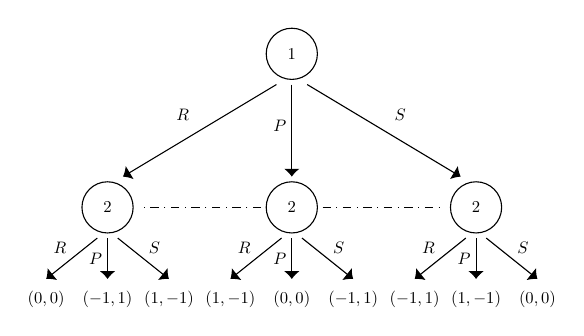
\begin{tikzpicture}[scale=0.13, every node/.style={scale=0.6}]
            \tikzstyle{every node}+=[inner sep=0pt]
                \draw [black] (36,-15) circle (2.5);
                \draw (36,-15) node {$1$};
                \draw [black] (36,-30) circle (2.5);
                \draw (36,-30) node {$2$};
                \draw [black] (54,-30) circle (2.5);
                \draw (54,-30) node {$2$};
                \draw [black] (18,-30) circle (2.5);
                \draw (18,-30) node {$2$};
                \draw (12,-39) node {$(0,0)$};
                \draw (18,-39) node {$(-1,1)$};
                \draw (24,-39) node {$(1,-1)$};
                \draw (30,-39) node {$(1,-1)$};
                \draw (36,-39) node {$(0,0)$};
                \draw (42,-39) node {$(-1,1)$};
                \draw (48,-39) node {$(-1,1)$};
                \draw (54,-39) node {$(1,-1)$};
                \draw (60,-39) node {$(0,0)$};
                \draw (26,-21) node [left] {$R$};
                \draw (36-0.5,-22) node [left] {$P$};
                \draw (46,-21) node [right] {$S$};
                \draw (14,-34) node [left] {$R$};
                \draw (18-0.5,-35) node [left] {$P$};
                \draw (22,-34) node [right] {$S$};
                \draw (32,-34) node [left] {$R$};
                \draw (36-0.5,-35) node [left] {$P$};
                \draw (40,-34) node [right] {$S$};
                \draw (50,-34) node [left] {$R$};
                \draw (54-0.5,-35) node [left] {$P$};
                \draw (58,-34) node [right] {$S$};
                \path [linedash] (39,-30) -- (51,-30);
                \path [linedash] (33,-30) -- (21,-30);
                \path [line] (36,-18) -- (36,-27);
                \path [line] (37.5,-18) -- (52.5,-27);
                \path [line] (34.5,-18) -- (19.5,-27);
                \path [line] (17,-33) -- (12,-37);
                \path [line] (18,-33) -- (18,-37);
                \path [line] (19,-33) -- (24,-37);
                \path [line] (35,-33) -- (30,-37);
                \path [line] (36,-33) -- (36,-37);
                \path [line] (37,-33) -- (42,-37);
                \path [line] (53,-33) -- (48,-37);
                \path [line] (54,-33) -- (54,-37);
                \path [line] (55,-33) -- (60,-37);
            \end{tikzpicture}
            \caption{Player 1 as root node}
            \label{fig:rps1}
    \end{subfigure}
    \vLine
    \begin{subfigure}{0.45\linewidth}
        \centering
        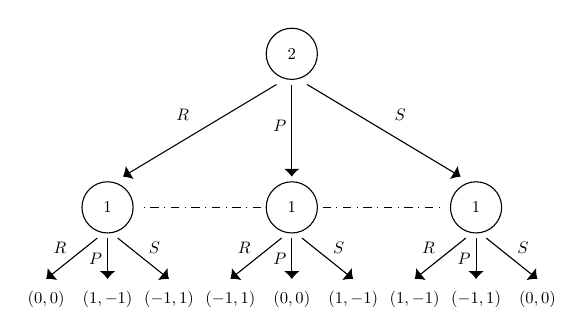
\begin{tikzpicture}[scale=0.13, every node/.style={scale=0.6}]
            \tikzstyle{every node}+=[inner sep=0pt]
                \draw [black] (36,-15) circle (2.5);
                \draw (36,-15) node {$2$};
                \draw [black] (36,-30) circle (2.5);
                \draw (36,-30) node {$1$};
                \draw [black] (54,-30) circle (2.5);
                \draw (54,-30) node {$1$};
                \draw [black] (18,-30) circle (2.5);
                \draw (18,-30) node {$1$};
                \draw (12,-39) node {$(0,0)$};
                \draw (18,-39) node {$(1,-1)$};
                \draw (24,-39) node {$(-1,1)$};
                \draw (30,-39) node {$(-1,1)$};
                \draw (36,-39) node {$(0,0)$};
                \draw (42,-39) node {$(1,-1)$};
                \draw (48,-39) node {$(1,-1)$};
                \draw (54,-39) node {$(-1,1)$};
                \draw (60,-39) node {$(0,0)$};
                \draw (26,-21) node [left] {$R$};
                \draw (36-0.5,-22) node [left] {$P$};
                \draw (46,-21) node [right] {$S$};
                \draw (14,-34) node [left] {$R$};
                \draw (18-0.5,-35) node [left] {$P$};
                \draw (22,-34) node [right] {$S$};
                \draw (32,-34) node [left] {$R$};
                \draw (36-0.5,-35) node [left] {$P$};
                \draw (40,-34) node [right] {$S$};
                \draw (50,-34) node [left] {$R$};
                \draw (54-0.5,-35) node [left] {$P$};
                \draw (58,-34) node [right] {$S$};
                \path [linedash] (39,-30) -- (51,-30);
                \path [linedash] (33,-30) -- (21,-30);
                \path [line] (36,-18) -- (36,-27);
                \path [line] (37.5,-18) -- (52.5,-27);
                \path [line] (34.5,-18) -- (19.5,-27);
                \path [line] (17,-33) -- (12,-37);
                \path [line] (18,-33) -- (18,-37);
                \path [line] (19,-33) -- (24,-37);
                \path [line] (35,-33) -- (30,-37);
                \path [line] (36,-33) -- (36,-37);
                \path [line] (37,-33) -- (42,-37);
                \path [line] (53,-33) -- (48,-37);
                \path [line] (54,-33) -- (54,-37);
                \path [line] (55,-33) -- (60,-37);
            \end{tikzpicture}
            \caption{Player 2 as root node}
            \label{fig:rps2}
    \end{subfigure}
    \caption{Game Tree of Rock Paper Scissors}
    \end{figure}
    Notice the similarity between both Game Trees. We will consider Figure \ref{fig:rps1} for following discussion.
    The Game can be written as
    \begin{itemize}
    \item $N = \{1, 2\}$
    \item $A_1 = A_2 = \{\text{Rock}, \text{Paper}, \text{Scissors}\}$, let's denote it as \{R, P, S\}
    \item $\mathbb{H} = \{(R, R), (R, P), (R, S), (P, R), (P, P), (P, S), (S, R), (S, P), (S, S)\}$
    \item $S_\mathbb{H} = \{\varepsilon, R, P, S\}$, where $\varepsilon$ denotes the empty history.
    \item $P(\varepsilon) = 1$, $P(R) = P(P) = P(S) = 2$
    \item $I_1 = \{\{\varepsilon\}\}$, $I_2 = \{\{R, P, S\}\}$
    \item $u_1(R, R) = 0$, $u_1(R, P) = -1$, $u_1(R, S) = 1$, $u_1(P, R) = 1$, $u_1(P, P) = 0$, $u_1(P, S) = -1$, $u_1(S, R) = -1$, $u_1(S, P) = 1$, $u_1(S, S) = 0$
    \item $u_2(R, R) = 0$, $u_2(R, P) = 1$, $u_2(R, S) = -1$, $u_2(P, R) = -1$, $u_2(P, P) = 0$, $u_2(P, S) = 1$, $u_2(S, R) = 1$, $u_2(S, P) = -1$, $u_2(S, S) = 0$
    \end{itemize}
\end{exm}
For detailed discussion on Extensive Form Games, refer Section \ref{sec:efg}
\subsection{Definitions}
Before we process, let's introduce some terms which will help in our understanding
\begin{defn}[Preferences]
    There can be many outcomes possible for game.
    Preferences of a player specify qualitatively the player's ranking of the different outcomes of the game.
\end{defn}
\begin{defn}[Utilities]
    Utilities are real valued payoffs that players receive when they play different actions.
    The utility of a player depends not only on the action played by that player but also on the actions played by the rest of the players.
\end{defn}
\begin{defn}[Utility function]
    The utility function or payoff function of a player is a real valued function defined on the set of all outcomes or strategy profiles.
    The utility function of each player maps multi-dimensional information (strategy profiles) into real numbers to capture preferences.
    \textbf{Von Neumann–Morgenstern utility theorem} establishes that there must exist a way of assigning real numbers to different strategy profiles in a way that the decision maker would always choose the option that maximizes her expected utility.
\end{defn}
\begin{defn}[Rationality]
    An agent is said to be rational if the agent always makes decisions in pursuit of her own objectives. One of the key assumptions in game theory is that the players are rational. That is, each agent’s objective is to maximize the expected value of her own payoff measured in some utility scale\footnote{Maximizing expected utility is not necessarily the same as maximizing expected
monetary returns.
In general, utility and money are nonlinearly related.
For example, a certain amount of money may provide different utilities to different players depending on how endowed or desperate they are.}.
    \begin{note}
       Depending on how the utility function is defined, rationality could mean self-interest, altruism, indifference, etc.
    \end{note}
\end{defn}
\begin{defn}[Intelligence]
    Intelligence means that each player in the game knows everything about the game that a game theorist knows, and the player is competent enough to make any inferences about the game that a game theorist can make.
    In particular, an intelligent player is \emph{strategic}, that is, would fully take into account his knowledge or expectation of behavior of other agents in determining what his optimal response should be.
    Such a strategy is called a \textbf{best response strategy}.
    \begin{note}
        Each player is assumed to have enough resources to carry out the required computations involved in determining a best response strategy.
    \end{note}
\end{defn}
\begin{defn}[Common Knowledge]
    A fact is common knowledge among the players if every player knows it, every player knows that every player knows it, and so on. That is, every statement of the form ``every player knows that every player knows that $\cdots$ every player knows it'' is true forever.
    \begin{note}
    In a strategic form game with complete information, $\langle N,(S_i),(u_i)\rangle$, the set $N$, the strategy sets $S_1,S_2,\ldots,S_n$ and the utility functions $u_1,u_2,\ldots,u_n$ are common knowledge.
    \end{note}
\end{defn}
\begin{defn}[Mutual Knowledge]
    If it happens that a fact is known to all the players, without the requirement of all players knowing that all players know it, etc., then such a fact is called mutual knowledge.
\end{defn}
\begin{defn}[Private Information]
    A player’s private information is any information that the player has that is not common knowledge or mutual knowledge among any of the players.
\end{defn}
\newpage
\part{Non-Cooperative Game Theory}
\section{Extensive Form Games}{\label{sec:efg}}
We have already seen the formal definition of Extensive Form Games (\ref{def:efg}).
The extensive form representation of a game provides a detailed and richly structured way to describe a game.
Specifically it captures:
\begin{itemize}
	\item who makes a move at any given time
	\item what actions each player may play
	\item what the players know before playing at each stage
	\item what the outcomes are as a function of the actions, and
	\item payoffs that players obtain from each outcome.
\end{itemize}
Extensive form games with a finite number of players and with a finite number of actions available to each player are depicted graphically using game trees.

In the game tree representation, the nodes are of three types:
\begin{itemize}
	\item root node (initial decision node)
	\item internal nodes (which are decision nodes)
	\item leaf nodes or terminal nodes (which are outcome nodes)
\end{itemize}
Each possible sequence of events that could occur in the game is captured by a path of links from the root node to one of the terminal nodes. When the game is played, the path that represents the sequence of events is called the \textbf{path of play}.
Each decision node is labeled with the player who takes a decision at that node.
Each decision node can be uniquely identified by a sequence of actions leading to that decision node from the root node.
Each node represents not only the current position in the game but also how it was reached.
The terminal nodes are labeled with the payoffs that the players would get in the outcomes corresponding to those nodes.

\subsection{Transforming Extensive Form to Strategic Form}
An extensive form game can be transformed into an equivalent strategic form game using the notion of a strategy.

$\mathbb{I}_i$ denotes the set of all information sets of player $i$ in the given game.
Let $A_i$ as usual denote the actions available to player $i$.
Given an information set $J \in \mathbb{I}_i$, let $C(J) \subseteq A_i$ be the set of all actions possible to player $i$ in the information set $J$. Then,
\begin{defn}[Strategy]
	A strategy $s_i$ of player $i$ is a mapping $s_i : \mathbb{I}_i \rightarrow A_i$ such that $s_i(J) \in C(J)\ \forall J \in I_i$.
\end{defn}
Shorthands for strategy profile
\begin{itemize}
	\item The index $-i$ is used to refer to all the players other than player $i$
	\item $s_{-i}$ is the strategy profile of all players other than player $i$
	\item Now, the complete strategy profile can be denoted as $(s_i, s_{-i})$
\end{itemize}
\begin{defn}[Outcome]
Given an extensive form game $\Gamma$ and a strategy profile $s = (s_1,\ldots,s_n)$ in the game, the outcome resulting out of the terminal history corresponding to the strategy profile $s$ is called the outcome of $s$ and is denoted by $O(s)$.
\end{defn}
\begin{note}
	Every extensive form game has a unique strategic form representation. The uniqueness is up to renaming or renumbering of strategies. We can also immediately observe that a given strategic form game may correspond to multiple extensive form games.
\end{note}
The strategy $s_i$ for player $i$ is a complete contingent plan that specifies an action for every information set of the player.
Let's dive into some examples.
\begin{exm}[Matching Pennies with Observation]{\label{exm:mp}}
	There are two players, 1 and 2, each of whom has a rupee coin.
	One of the players puts down his rupee coin heads or tails up.
	The other player sees the outcome and puts down her coin heads up or tails up.
	If both the coins show heads or both the coins show tails, player 2 gives one rupee to player 1.
	If one of the coins shows heads and the other coin shows tails player 1 gives one rupee to player 2.

	Depending on whether player 1 or player 2 moves first, there are two versions of this game. Figure \ref{fig:mpwo1} shows the game tree when player 1 moves first while Figure \ref{fig:mpwo2} shows the game tree when player 2 moves first.
	\begin{figure}[H]
		\centering
		\begin{subfigure}{0.45\linewidth}
		        \centering
		        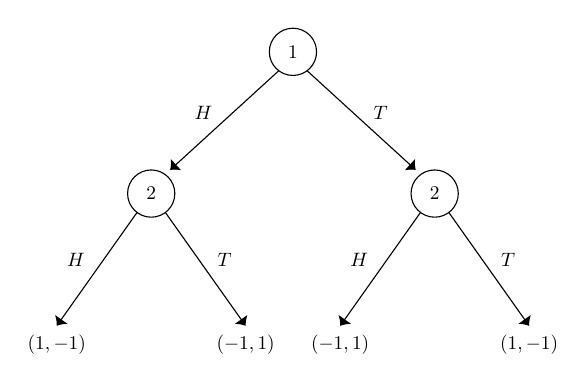
\begin{tikzpicture}[scale=0.12, every node/.style={scale=0.7}]
		            \tikzstyle{every node}+=[inner sep=0pt]
		                \draw [black] (0,30) circle (2.5);
		                \draw (0,30) node {$1$};
		                \draw [black] (-15,15) circle (2.5);
		                \draw (-15,15) node {$2$};
		                \draw [black] (15,15) circle (2.5);
		                \draw (15,15) node {$2$};;
		                \draw (-25,-1) node {$(1,-1)$};
		                \draw (-5,-1) node {$(-1,1)$};
		                \draw (5,-1) node {$(-1,1)$};
		                \draw (25,-1) node {$(1,-1)$};
		                \draw (-8.5,23.5) node [left] {$H$};
		                \draw (8.5,23.5) node [right] {$T$};
		                \draw (-22,8) node [left] {$H$};
		                \draw (-8,8) node [right] {$T$};
		                \draw (8,8) node [left] {$H$};
		                \draw (22,8) node [right] {$T$};
		                \path [line] (-1.5,28) -- (-13,17.5);
		                \path [line] (1.5,28) -- (13,17.5);
		                \path [line] (-16.5,13) -- (-25,1);
		                \path [line] (-13.5,13) -- (-5,1);
		                \path [line] (13.5,13) -- (5,1);
		                \path [line] (16.5,13) -- (25,1);
		            \end{tikzpicture}
		            \caption{Player 1 moves first}
		            \label{fig:mpwo1}
		    \end{subfigure}
		    \vLine
		    \begin{subfigure}{0.45\linewidth}
		        \centering
		        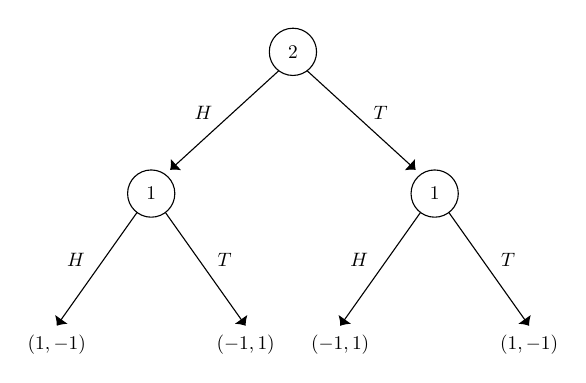
\begin{tikzpicture}[scale=0.12, every node/.style={scale=0.7}]
		            \tikzstyle{every node}+=[inner sep=0pt]
		                \draw [black] (0,30) circle (2.5);
		                \draw (0,30) node {$2$};
		                \draw [black] (-15,15) circle (2.5);
		                \draw (-15,15) node {$1$};
		                \draw [black] (15,15) circle (2.5);
		                \draw (15,15) node {$1$};;
		                \draw (-25,-1) node {$(1,-1)$};
		                \draw (-5,-1) node {$(-1,1)$};
		                \draw (5,-1) node {$(-1,1)$};
		                \draw (25,-1) node {$(1,-1)$};
		                \draw (-8.5,23.5) node [left] {$H$};
		                \draw (8.5,23.5) node [right] {$T$};
		                \draw (-22,8) node [left] {$H$};
		                \draw (-8,8) node [right] {$T$};
		                \draw (8,8) node [left] {$H$};
		                \draw (22,8) node [right] {$T$};
		                \path [line] (-1.5,28) -- (-13,17.5);
		                \path [line] (1.5,28) -- (13,17.5);
		                \path [line] (-16.5,13) -- (-25,1);
		                \path [line] (-13.5,13) -- (-5,1);
		                \path [line] (13.5,13) -- (5,1);
		                \path [line] (16.5,13) -- (25,1);
		            \end{tikzpicture}
		            \caption{Player 2 moves first}
		            \label{fig:mpwo2}
		    \end{subfigure}
		% \begin{subfigure}{0.45\linewidth}
		% 	\centering
		% 	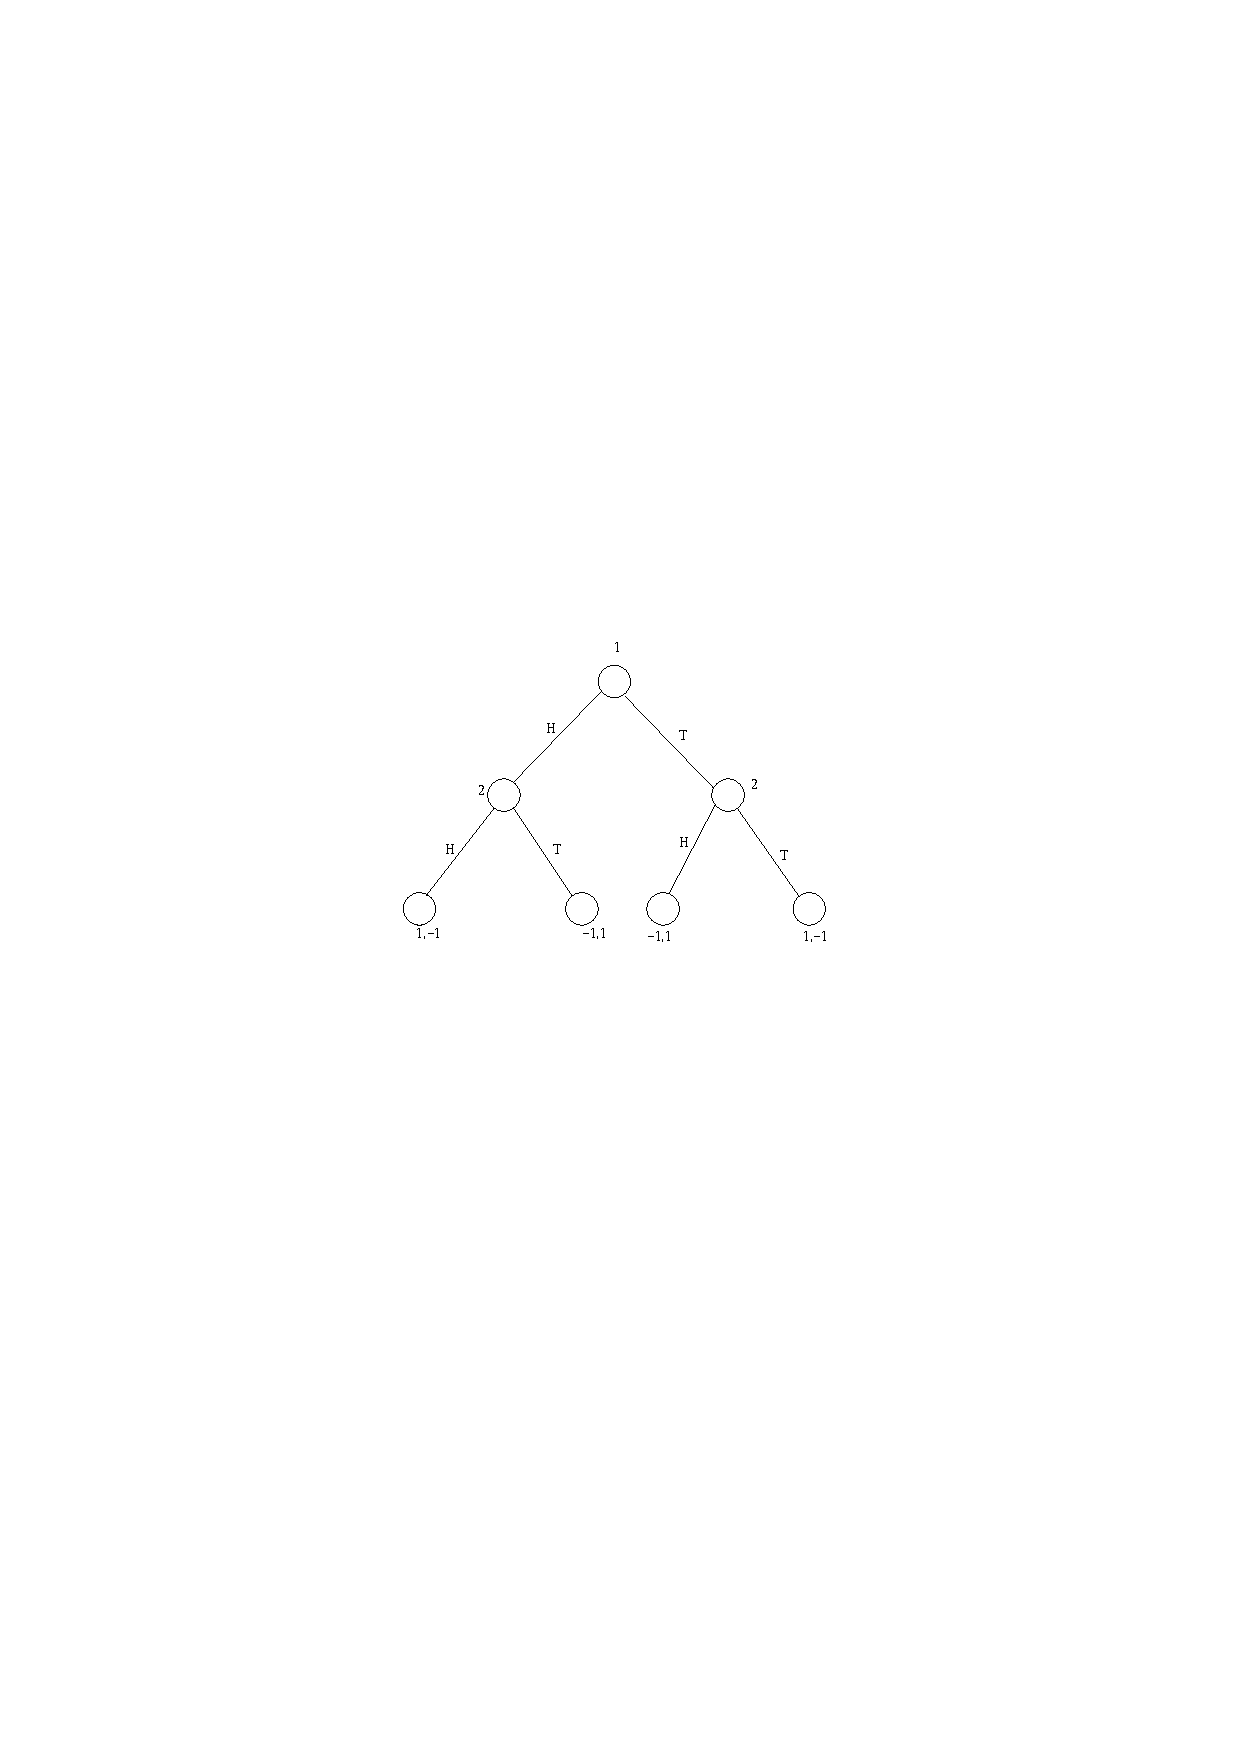
\includegraphics[width=\linewidth]{mpwo1.pdf}
		% 	\caption{Player 1 moves first}
		% 	\label{fig:mpwo1}
		% \end{subfigure}
		% \vLine
		% \begin{subfigure}{0.45\linewidth}
		% 	\centering
		% 	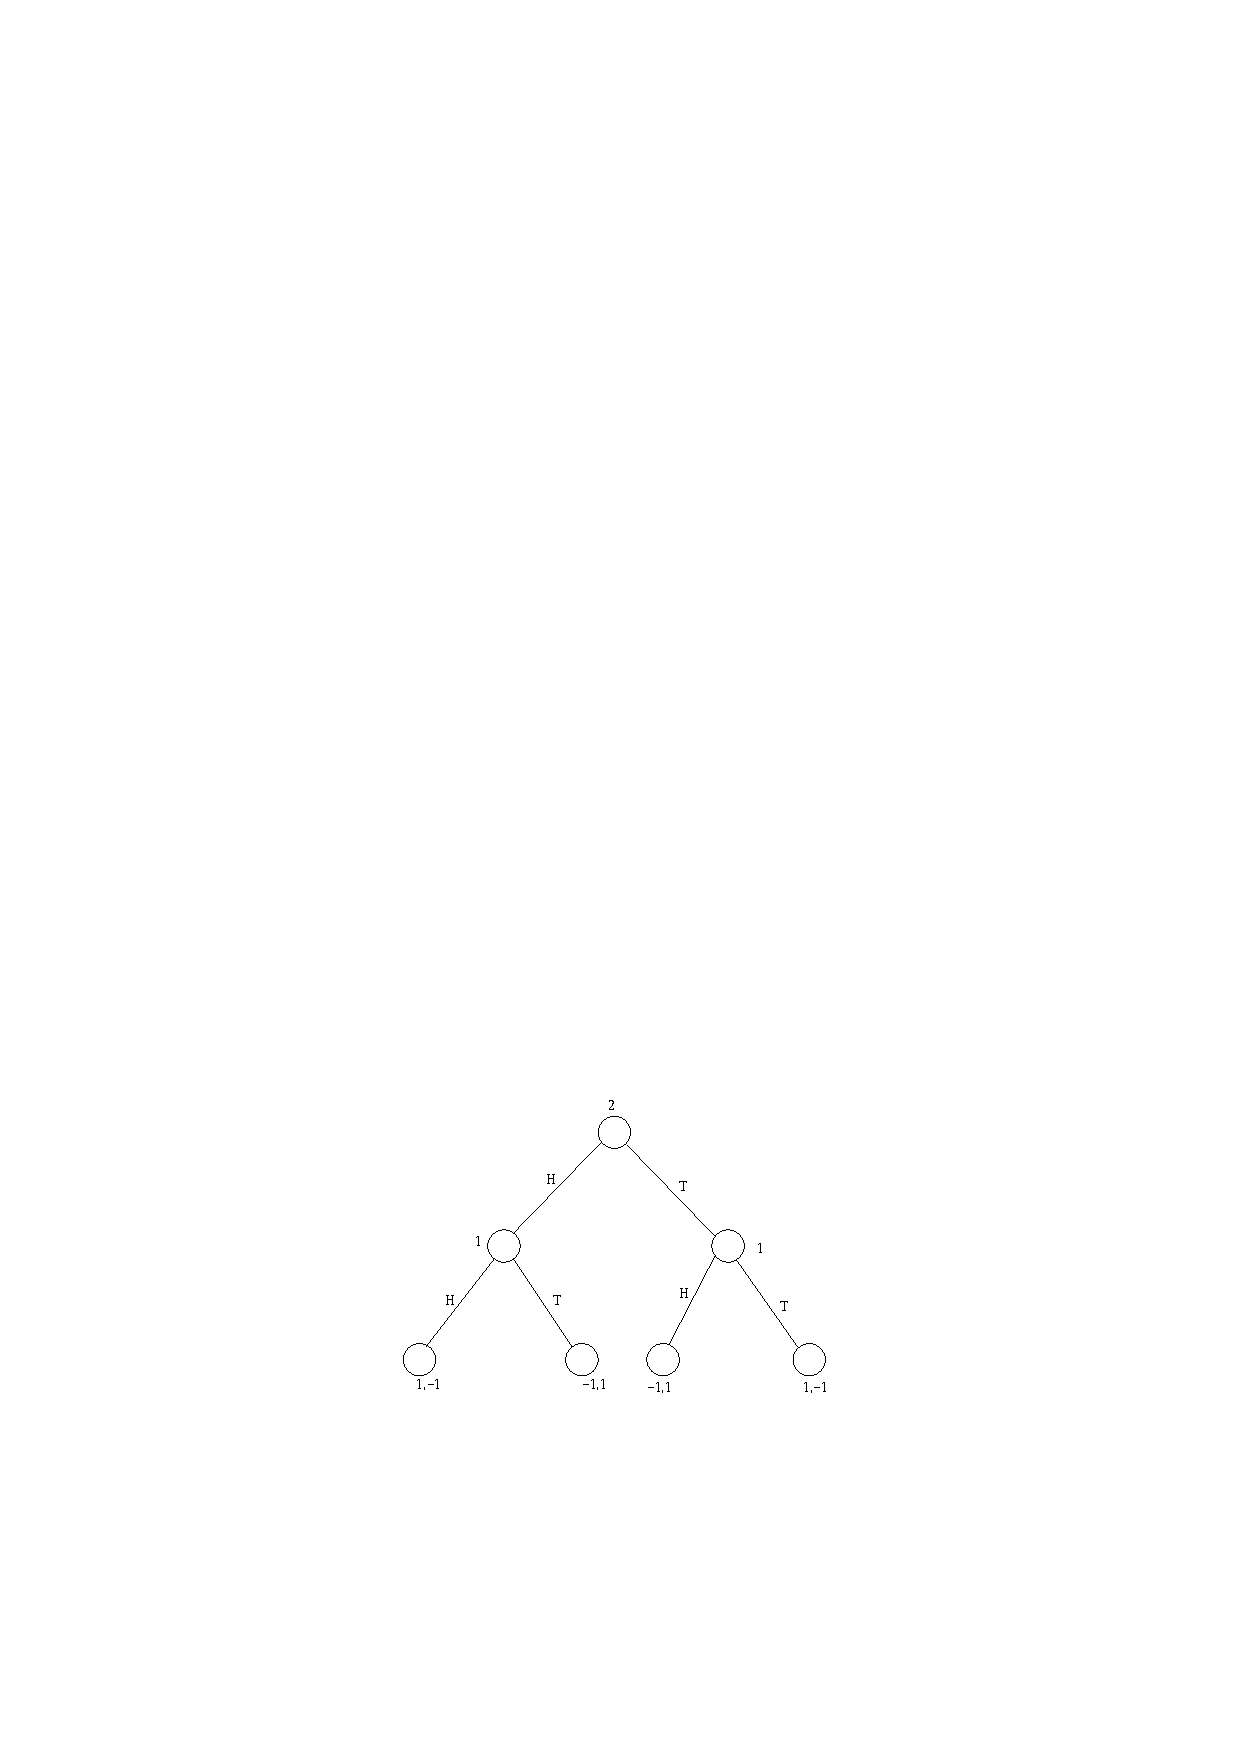
\includegraphics[width=\linewidth]{mpwo2.pdf}
		% 	\caption{Player 2 moves first}
		% 	\label{fig:mpwo2}
		% \end{subfigure}
		\caption{Matching pennies game with observation}
		\label{fig:mpwo}
	\end{figure}
	For this game in Figure \ref{fig:mpwo1}, we have
	\[N = \{1, 2\}\]
	\[A_1 = A_2	 = \{H, T\}\]
	\[\mathbb{H} = \{(H,H), (H, T), (T,H), (T, T)\}\]
	\[S_\mathbb{H} = \{\varepsilon,H, T\}\]
	\[P(\varepsilon) = 1; P(H) = 2;\quad P(T) = 2\]
	\[\mathbb{I}_1 = \{\{\varepsilon\}\};\quad \mathbb{I}_2 = \{\{H\}, \{T\}\}\]
	\[u_1(HH) = 1;\quad u_1(HT) = -1;\quad u_1(TH) = -1;\quad u_1(TT) = 1\]
	\[u_2(HH) = -1;\quad u_2(HT) = 1;\quad u_2(TH) = 1;\quad u_2(TT) = -1\]
	Strategies of player 1 are $s_{11}: {\varepsilon}\rightarrow H$ and $s_{12}: {\varepsilon}\rightarrow T$, similarly for player 2 

	$s_{21}: {H}\rightarrow H; {T}\rightarrow H$, $s_{22}: {H}\rightarrow H; {T}\rightarrow T$, $s_{23}: {H}\rightarrow T; {T}\rightarrow H$ and $s_{24}: {H}\rightarrow T; {T}\rightarrow T$
\end{exm}
\begin{table}[H]
    \centering
    \subfloat[With Observation]{
    \begin{tabular}{ |c|c|c|c|c| } 
        \hline
        1/2 & $s_{21}$ & $s_{22}$ & $s_{23}$ & $s_{24}$\\\hline
        $s_{11}$ & $1,-1$ & $1,-1$ & $-1,1$ & $-1,1$\\\hline
        $s_{12}$ & $-1,1$ & $1,-1$ & $-1,1$ & $1,-1$\\\hline
    \end{tabular}}
\vLine
    \subfloat[Without Observation]{
    \begin{tabular}{ |c|c|c| } 
        \hline
        1/2 & $s_{21}$ & $s_{22}$\\\hline
        $s_{11}$ & $1,-1$ & $-1,1$ \\\hline
        $s_{12}$ & $-1,1$ & $1,-1$\\\hline
    \end{tabular}}
    \caption{Payoff Matrix for Matching Pennies}
\end{table}
\begin{exm}[Matching Pennies without Observation]
	In this case, one of the players places his rupee coin heads up or tails up.
	The other player does not observe the outcome and only puts down her rupee coin heads up or tails up. This is equivalent to the two players put down their rupee coins simultaneously.
	Depending on whether player 1 or player 2 moves first, there are two versions of this game. Figure \ref{fig:mpwoo1} shows the game tree when player 1 moves first while Figure \ref{fig:mpwoo2} shows the game tree when player 2 moves first.
	\begin{figure}[h]
		\centering
		\begin{subfigure}{0.45\linewidth}
		        \centering
		        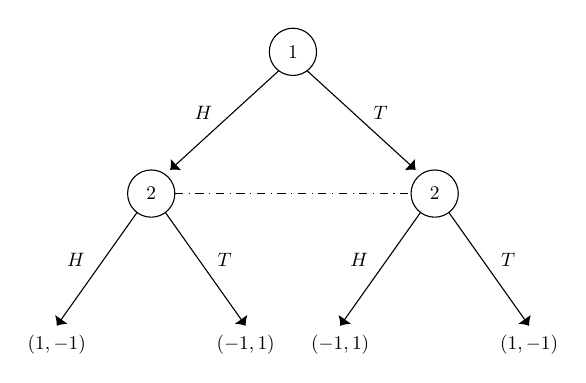
\begin{tikzpicture}[scale=0.12, every node/.style={scale=0.7}]
		            \tikzstyle{every node}+=[inner sep=0pt]
		                \draw [black] (0,30) circle (2.5);
		                \draw (0,30) node {$1$};
		                \draw [black] (-15,15) circle (2.5);
		                \draw (-15,15) node {$2$};
		                \draw [black] (15,15) circle (2.5);
		                \draw (15,15) node {$2$};;
		                \draw (-25,-1) node {$(1,-1)$};
		                \draw (-5,-1) node {$(-1,1)$};
		                \draw (5,-1) node {$(-1,1)$};
		                \draw (25,-1) node {$(1,-1)$};
		                \draw (-8.5,23.5) node [left] {$H$};
		                \draw (8.5,23.5) node [right] {$T$};
		                \draw (-22,8) node [left] {$H$};
		                \draw (-8,8) node [right] {$T$};
		                \draw (8,8) node [left] {$H$};
		                \draw (22,8) node [right] {$T$};
		                \path [linedash] (-12.5,15) -- (12.5,15);
		                \path [line] (-1.5,28) -- (-13,17.5);
		                \path [line] (1.5,28) -- (13,17.5);
		                \path [line] (-16.5,13) -- (-25,1);
		                \path [line] (-13.5,13) -- (-5,1);
		                \path [line] (13.5,13) -- (5,1);
		                \path [line] (16.5,13) -- (25,1);
		            \end{tikzpicture}
		            \caption{Player 1 moves first}
		            \label{fig:mpwoo1}
		    \end{subfigure}
		    \vLine
		    \begin{subfigure}{0.45\linewidth}
		        \centering
		        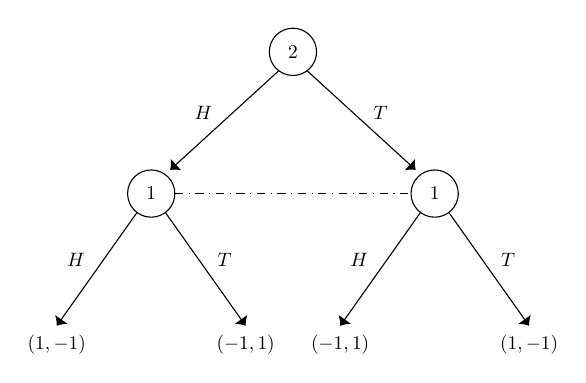
\begin{tikzpicture}[scale=0.12, every node/.style={scale=0.7}]
		            \tikzstyle{every node}+=[inner sep=0pt]
		                \draw [black] (0,30) circle (2.5);
		                \draw (0,30) node {$2$};
		                \draw [black] (-15,15) circle (2.5);
		                \draw (-15,15) node {$1$};
		                \draw [black] (15,15) circle (2.5);
		                \draw (15,15) node {$1$};;
		                \draw (-25,-1) node {$(1,-1)$};
		                \draw (-5,-1) node {$(-1,1)$};
		                \draw (5,-1) node {$(-1,1)$};
		                \draw (25,-1) node {$(1,-1)$};
		                \draw (-8.5,23.5) node [left] {$H$};
		                \draw (8.5,23.5) node [right] {$T$};
		                \draw (-22,8) node [left] {$H$};
		                \draw (-8,8) node [right] {$T$};
		                \draw (8,8) node [left] {$H$};
		                \draw (22,8) node [right] {$T$};
		                \path [linedash] (-12.5,15) -- (12.5,15);
		                \path [line] (-1.5,28) -- (-13,17.5);
		                \path [line] (1.5,28) -- (13,17.5);
		                \path [line] (-16.5,13) -- (-25,1);
		                \path [line] (-13.5,13) -- (-5,1);
		                \path [line] (13.5,13) -- (5,1);
		                \path [line] (16.5,13) -- (25,1);
		            \end{tikzpicture}
		            \caption{Player 2 moves first}
		            \label{fig:mpwoo2}
		    \end{subfigure}
		\caption{Matching pennies game without observation}
		\label{fig:mpwoo}
	\end{figure}
	% \begin{figure}[H]
	% 	\centering
	% 	\begin{subfigure}{0.45\linewidth}
	% 		\centering
	% 		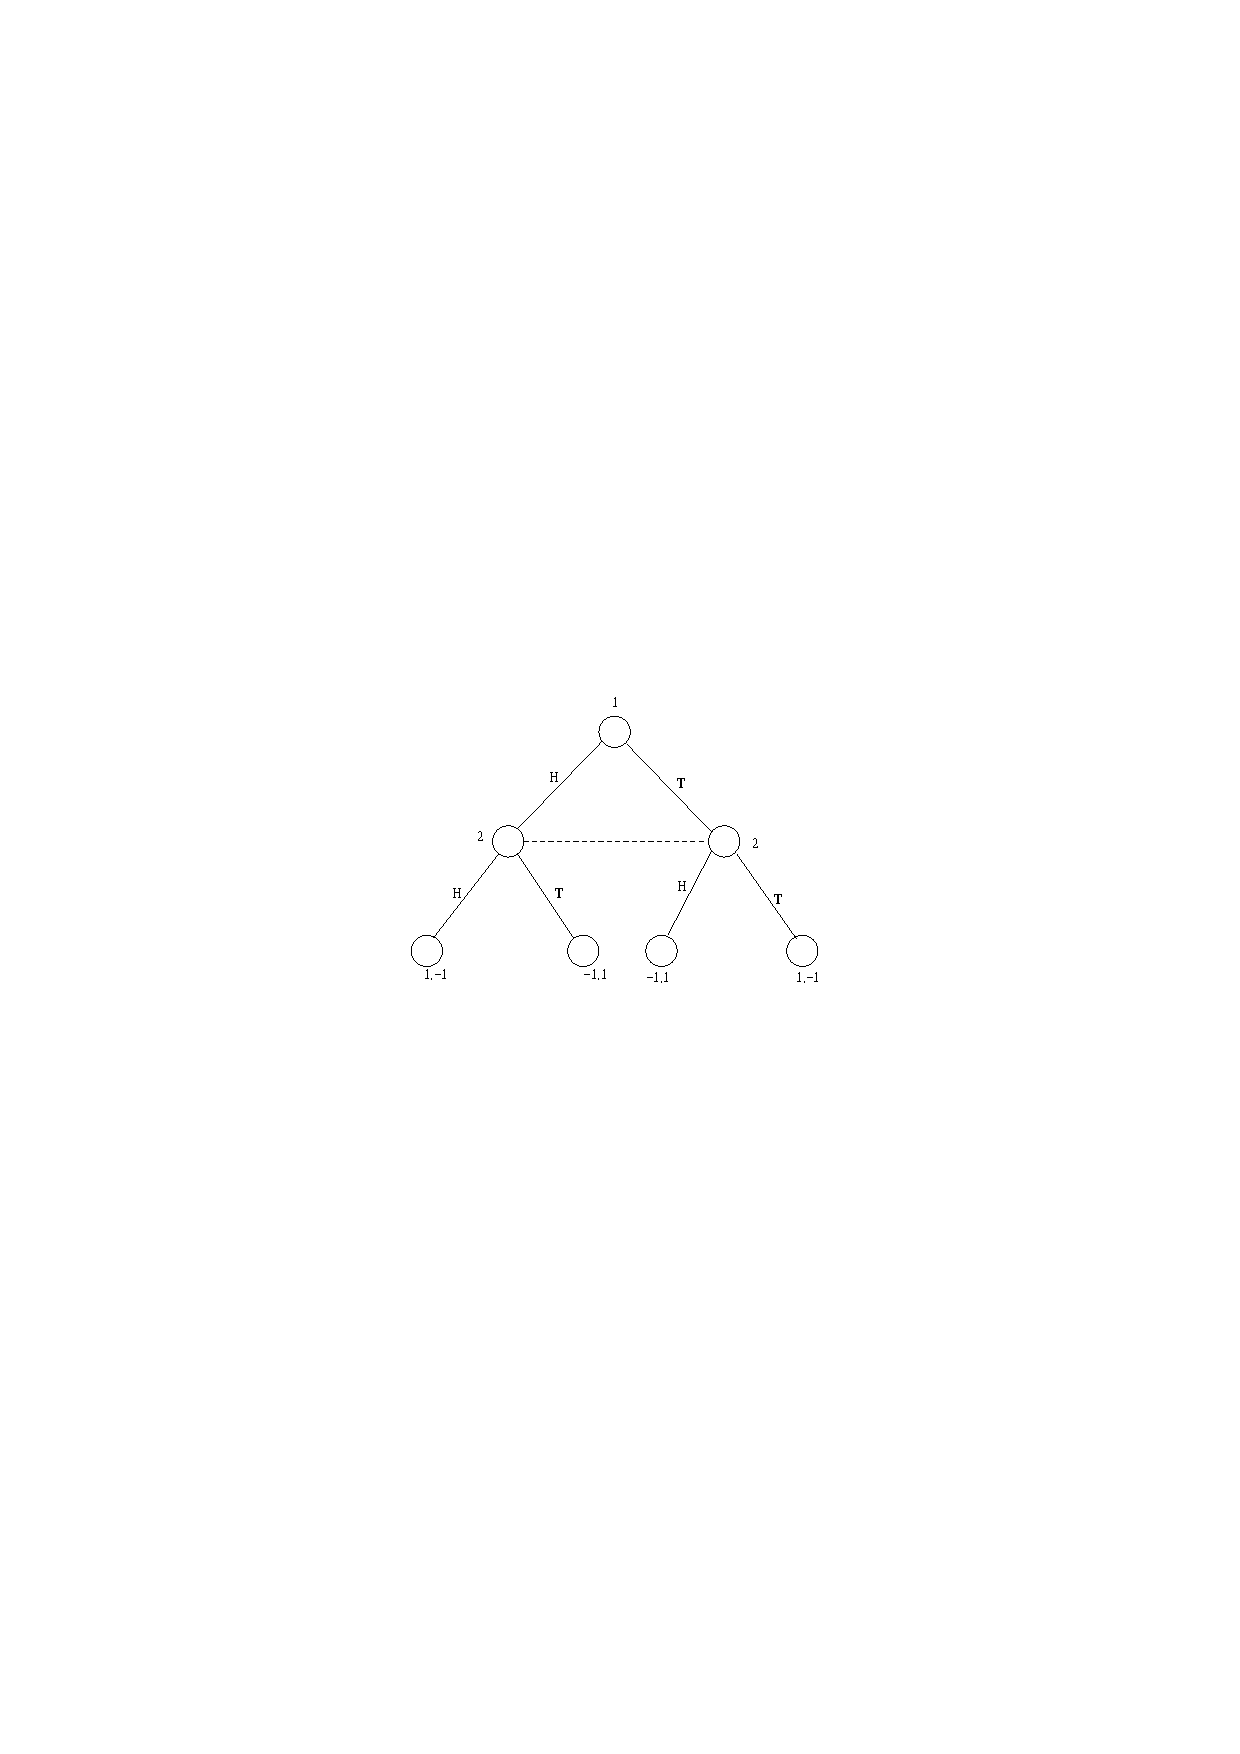
\includegraphics[width=\linewidth]{mpwoo1.pdf}
	% 		\caption{Player 1 moves first}
	% 		\label{fig:mpwoo1}
	% 	\end{subfigure}
	% 	\vLine
	% 	\begin{subfigure}{0.45\linewidth}
	% 		\centering
	% 		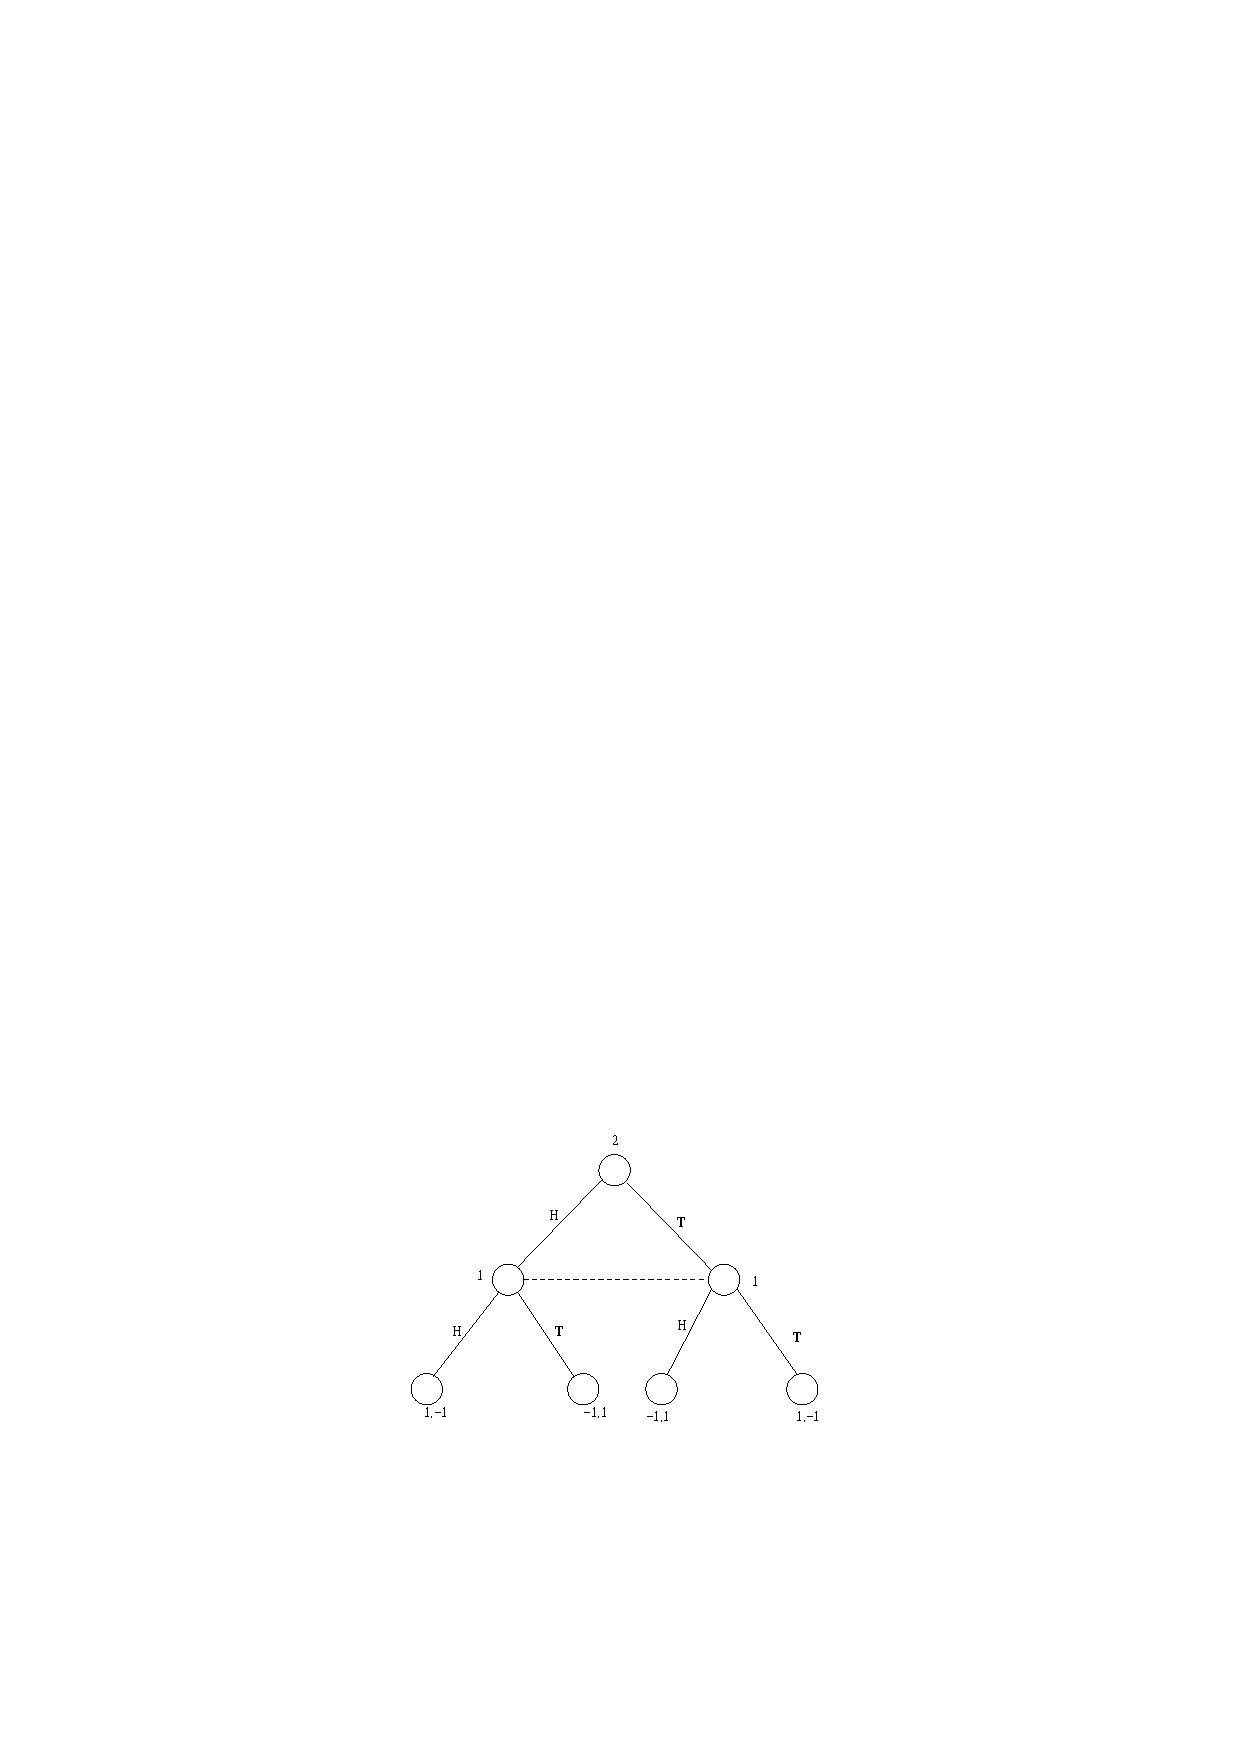
\includegraphics[width=\linewidth]{mpwoo2.pdf}
	% 		\caption{Player 2 moves first}
	% 		\label{fig:mpwoo2}
	% 	\end{subfigure}
	% 	\caption{Matching pennies game without observation when player 1 moves first}
	% 	\label{fig:mpwoo}
	% \end{figure}
	Note that the game trees of Figures \ref{fig:mpwo1} and \ref{fig:mpwoo1} are virtually the same except that the two decision nodes corresponding to player 2 in Figure \ref{fig:mpwoo1} are connected with dotted lines. Same case with Figures \ref{fig:mpwo2} and \ref{fig:mpwoo2}
	\begin{defn}[Information Set]
		An information set of a player is a set of that player's decision nodes that are indistinguishable to her.
		Since each decision node corresponds uniquely to a sequence of actions from the root node to the decision node, each information set of a player consists of all proper subhistories relevant to that player which are indistinguishable to that player. 
	\end{defn}
\end{exm}
\begin{note}
	Though the action sets of players can be deduced from terminal histories and the player function, we explicitly include action sets as a part of definition of an extensive form game for ease of understanding.
\end{note}
\begin{defn}[Perfect Information and Imperfect Information Games]
	An extensive form game with perfect information is one in which all the information sets are singletons.
	If at least one information set of at least one player has two or more elements, the game is said to be of imperfect information.
\end{defn}
In a game with perfect information, each player is able to observe all previous moves or the entire history thus far.
Each player knows precisely where she is currently and also knows precisely how she has reached that node.

Games in Figures \ref{fig:mpwo1} and \ref{fig:mpwo2} are games with perfect information while the games shown in Figures \ref{fig:mpwoo1} and \ref{fig:mpwoo2} are games with imperfect information.
\section{Strategic Form Games}{\label{sec:sfg}}
We have already seen the formal definition of Strategic Form Games (\ref{def:sfg}).

The idea behind the strategic form representation is that a player's decision problem is to essentially choose a strategy that will counter most effectively the strategies adopted by the other players.
Such a strategy is called a best response strategy which is formally defined as follows.
\begin{defn}[Best Response Strategy]
    Given a strategic form game $\Gamma = \langle N,(S_i),(u_i)\rangle$ and a strategy profile $s_{-i} \in S_{-i}$, we say $s_i \in S_{i}$ is a best response strategy of player $i$ with respect to $s_{-i}$ if
    \[u_i(s_i,s_{-i})\geq u_i(s^\prime_i,s_{-i})\ \forall s^\prime_i \in S_i\]
\end{defn}
\subsection{Prisoner's Dilemma Game}
This is one of the most extensively studied problems in game theory, with many interesting interpretations in a wide variety of situations.
You might have realised that the cover page of my report depicts this game.

Bill and Bob are arrested for allegedly committing a crime and are lodged in separate cells.
The interrogator questions them separately.
The interrogator privately tells each prisoner that if he is the only one to confess, he will get a light sentence of 1 year in jail while the other would be sentenced to 10 years in jail.
If both players confess, they would get 3 years each in jail.
If neither confesses, then each would get 2 years in jail.
The interrogator also informs each prisoner what has been told to the other prisoner.
\begin{table}[h]{\label{tab:pd}}
\centering
	\begin{tabular}{ |c|c|c| } 
        \hline
        Bill (1)/ Bob (2) & $NC$ & $C$\\\hline
        $NC$ & $-2,-2$ & $-10,-1$ \\\hline
        $C$ & $-1,-10$ & $-3,-3$\\\hline
    \end{tabular}
    \caption{Payoff Matrix for Prisoner's Dilemma}
\end{table}
Here, Bill would like to play a strategy that offers a best response to a best response strategy that the Bob may adopt, Bob also would like to play a strategy that offers a best response to the Bill's best response strategy.

We notice that $(C,C)$ is each player's best response strategy regardless of what the other player plays:
\[u_1(C,C)=-3>u_1(NC,C)=-10\quad u_1(C,NC)=-1>u_1(NC,NC)=-2\]
\[u_2(C,C)=-3>u_2(C,NC)=-10\quad u_2(NC,C)=-1>u_2(NC,NC)=-2\]
Thus $(C, C)$ is a natural prediction for this game.
However, the outcome $(NC,NC)$ is the best outcome jointly for the players.
Prisoner’s dilemma is a classic example of a game where rational, intelligent behavior does not lead to an outcome where the sum of utilities of the players is maximal.
Also, each prisoner has a negative effect or externality on the other.
When a prisoner moves away from $(NC,NC)$ to reduce his jail term by 1 year, the jail term of the other prisoner increases by 8 years.
\section{Dominant Strategy Equilibria}
We start the section with the notion of strong dominance.
Subsequently, we introduce the notions of weak dominance and very weak dominance.
\subsection{Strong Dominance}
\begin{defn}[Strongly Dominated Strategy]
    Given a strategic form game $\Gamma = \langle N,(S_i),(u_i)\rangle$, a strategy $s_i \in S_i$ of player $i$ is said to be strongly dominated by another strategy $s^\prime_i \in S_i$
    \[u_i(s^\prime_i,s_{-i})> u_i(s_i,s_{-i})\ \forall s_{-i} \in S_{-i}\]
\end{defn}
We also say strategy $s^\prime_i$ strongly dominates strategy $s_i$.
\begin{defn}[Strongly Dominant Strategy]
    A strategy $s^*_i \in S_i$ is said to be strongly dominant for player $i$ if it strongly dominates every other strategy $s_i \in S_i$.
    That is $\forall s_i\neq s_i^*,$
    \[u_i(s^*_i,s_{-i})> u_i(s_i,s_{-i})\ \forall s_{-i} \in S_{-i}\]
\end{defn}
\begin{defn}[Strongly Dominant Strategy Equilibrium]
    A strategy profile $(s_1^*,s_2^*,\ldots,s_n^*)$ is called a strongly dominated strategy equilibrium of the game $\Gamma = \langle N,(S_i),(u_i)\rangle$ if, $\forall i=1,2,\ldots,n$, the strategy $s_i^*$ is a strongly dominated strategy for player $i$.
\end{defn}
Clearly, if a (rational) player has a strongly dominant strategy, then we should expect the player to choose that strategy.
On the other hand, if a player has a strongly dominated strategy, then we should expect the player not to play it.

Recall, Prisoner's Dilemma, $C$ is a strongly dominant strategy for Bill and also for Bob. Therefore $(C, C)$ is a \textbf{strongly dominant strategy equilibrium} for this game.
\subsection{Weak Dominance}
\begin{defn}[Weakly Dominated Strategy]
    A strategy $s_i \in S_i$ of player $i$ is said to be weakly dominated by another strategy $s^\prime_i \in S_i$
    \[u_i(s^\prime_i,s_{-i})\geq u_i(s_i,s_{-i})\ \forall s_{-i} \in S_{-i}\quad \text{and}\quad u_i(s^\prime_i,s_{-i})> u_i(s_i,s_{-i})\ \text{for some} s_{-i} \in S_{-i}\]
\end{defn}
The strategy $s^\prime_i$ weakly dominates strategy $s_i$.

The strict inequality is to be satisfied for at least one $s_{-i}$.
\begin{defn}[Weakly Dominant Strategy]
    A strategy $s^*_i \in S_i$ is said to be weakly dominant for player $i$ if it weakly dominates every other strategy $s_i \in S_i$.
\end{defn}
\begin{defn}[Weakly Dominant Strategy Equilibrium]
    A strategy profile $(s_1^*,s_2^*,\ldots,s_n^*)$ is called a weakly dominated strategy equilibrium of the game $\Gamma = \langle N,(S_i),(u_i)\rangle$ if, $\forall i=1,2,\ldots,n$, the strategy $s_i^*$ is a weakly dominated strategy for player $i$.
\end{defn}
\subsection{Very Weak Dominance}
\begin{defn}[Very Weakly Dominated Strategy]
    A strategy $s_i \in S_i$ of player $i$ is said to be very weakly dominated by another strategy $s^\prime_i \in S_i$
    \[u_i(s^\prime_i,s_{-i})\geq u_i(s_i,s_{-i})\ \forall s_{-i} \in S_{-i}\]
\end{defn}
The strategy $s^\prime_i$ very weakly dominates strategy $s_i$.

Here, the strict inequality need not be satisfied for any $s_{-i}$ unlike in the case of weak dominance where strict inequality must be satisfied for at least one $s_{-i}$.
\begin{defn}[Very Weakly Dominant Strategy]
    A strategy $s^*_i \in S_i$ is said to be very weakly dominant for player $i$ if it very weakly dominates every other strategy $s_i \in S_i$.
\end{defn}
\begin{defn}[Very Weakly Dominant Strategy Equilibrium]
    A strategy profile $(s_1^*,s_2^*,\ldots,s_n^*)$ is called a very weakly dominated strategy equilibrium of the game $\Gamma = \langle N,(S_i),(u_i)\rangle$ if, $\forall i=1,2,\ldots,n$, the strategy $s_i^*$ is a very weakly dominated strategy for player $i$.
\end{defn}
\begin{table}[H]
\centering
	\subfloat[Here $C$ is a weakly dominant strategy.\newline So, $(C,C)$ is weakly dominant strategy equilibrium]{
    \begin{tabular}{ |c|c|c| } 
        \hline
        Bill (1)/ Bob (2) & $NC$ & $C$\\\hline
        $NC$ & $-2,-2$ & $-10,-2$ \\\hline
        $C$ & $-2,-10$ & $-5,-5$\\\hline
    \end{tabular}}
    \vLine
    \subfloat[Here $C$ and $NC$ are very weakly dominant strategies.\newline So, all 4 strategy profiles are very weakly dominant strategy equilibrium]{
    \begin{tabular}{ |c|c|c| } 
        \hline
        Bill (1)/ Bob (2) & $NC$ & $C$\\\hline
        $NC$ & $-2,-2$ & $-5,-2$ \\\hline
        $C$ & $-2,-10$ & $-5,-10$\\\hline
    \end{tabular}}
    \caption{Payoff Matrix for Modified Prisoner's Dilemma}
\end{table}
Dominant strategy equilibria (strongly dominant, weakly dominant, very weakly dominant), if they exist, are very desirable, however, rarely do they exist because the conditions to be satisfied are quite demanding.
A dominant strategy equilibrium requires that each player’s strategy be a best response strategy against all possible strategy choices of the other players.
\section{Pure Strategy Nash Equilibria}
We get the notion of Nash equilibrium, a central notion in game theory, if we only insist that each player’s strategy offers a best response against the Nash equilibrium strategies of the other players.
This solution concept is named after John Nash, one of the most celebrated game theorists of our times.
\subsection{The Notion of Nash Equilibrium}
\begin{defn}[Pure Strategy Nash Equilibrium]
	Given a strategic form game $\Gamma = \langle N,(S_i),(u_i)\rangle$, the strategy profile $s^*=(s_1^*,s_2^*,\ldots,s_n^*)$ is called a pure strategy Nash equilibrium of $\Gamma$ if
	\[u_i(s^*_i,s^*_{-i})\geq u_i(s_i,s^*_{-i})\ \forall s_{i} \in S_{i}\ \forall i=1,2,\ldots,n\]
	Alternatively,
	\[u_i(s^*_i,s^*_{-i})= \underbrace{\op{max}}_{s_{i} \in S_{i}} u_i(s_i,s^*_{-i})\ \forall i=1,2,\ldots,n\]
	That is, each player’s Nash equilibrium strategy is a best response to the Nash equilibrium strategies of the other players
\end{defn}
Another alternate way of describing a pure strategy Nash equilibrium (PSNE).
\begin{defn}[Best Response Correspondence]{\label{def:brc}}
	Given a strategic form game $\Gamma = \langle N,(S_i),(u_i)\rangle$,the best response correspondence for player $i$ is the mapping $b_i : S_{-i} \rightarrow 2^{S_i}$ defined by
	\[b_i(s_{-i}) = \{s_i \in S_i : u_i(s_i, s{-i}) \geq u_i(s^\prime_i, s{-i}) \ \forall\  s^\prime_i \in S_i\}\]
	It can be seen that the strategy profile $(s_1^*,s_2^*,\ldots,s_n^*)$ is a pure strategy Nash equilibrium iff
	\[s^*_i \in b_i(s^*_{-i}), \forall i = 1,\ldots, n\]
\end{defn}
Again recall Prisoner's Dilemma (Table 3.
%\ref{tab:pd}
) :p, $(C, C)$ is the unique Nash equilibrium here.
To see why, we have to just look at the best response sets:
\[b_1(C) = \{C\};\quad b_1(NC) = \{C\};\quad b_2(C) = \{C\};\quad b_2(NC) = \{C\}\]
Since $(s^*_1, s^*_2)$ is a pure strategy Nash equilibrium iff $s^*_1 \in b_1(s^*_2)$ and $s^*_2 \in b_2(s^*_1)$, the only
possible pure strategy Nash equilibrium here is $(C, C)$.
In fact as already seen, this is a strongly dominant strategy equilibrium.
\begin{rem}
	Given a strategic form game $\Gamma = \langle N,(S_i),(u_i)\rangle$, a strongly (weakly) (very weakly) dominant strategy equilibrium $(s_1^*,\ldots,s_n^*)$ is also a Nash equilibrium.

	In a dominant strategy equilibrium, the equilibrium strategy of each player offers a best response irrespective of the strategies of the rest of the players.
	In a pure strategy Nash equilibrium, the equilibrium strategy of each player offers a best response against the Nash equilibrium strategies of the rest of the players.
	Thus, Nash equilibrium is a \textbf{much weaker notion of equilibrium} than a dominant strategy equilibrium.
\end{rem}
\begin{note}
	A Nash equilibrium need not be a dominant strategy equilibrium.
\end{note}
\subsection{Games without a Pure Strategy Nash Equilibrium}
Given a strategic form game, there is no guarantee that a pure strategy Nash equilibrium will exist.

Recall Matching Pennies Game (Example \ref{exm:mp}), it is easy to see that this game does not have a pure strategy Nash equilibrium.
The Rock Paper Scissors (Example \ref{exm:rps}) game also does not have a Nash equilibrium.
\subsection{Interpretations of Nash Equilibrium}
\subsubsection{Prescription}
Here we see interesting interpretations of Nash equilibrium.
An adviser or a consultant to the n players would logically prescribe a Nash equilibrium strategy profile to the players.
If the adviser recommends strategies that do not constitute a Nash equilibrium, then at least one player would find she is better off doing differently than advised.
If the adviser prescribes strategies that do constitute a Nash equilibrium, then the players are happy because playing the prescribed strategy is best under the assumption that the other players will play their prescribed strategies.
Thus a logical, rational, adviser would recommend a Nash equilibrium profile to the players.
\subsubsection{Prediction}
If the players are rational and intelligent, then a Nash equilibrium provides one possible, scientific prediction for the game.
For example, a systematic elimination of strongly dominated strategies will lead to a reduced form that will include a Nash equilibrium %see section later
\subsubsection{Self-Enforcing Agreement}
A Nash equilibrium can be viewed as an implicit or explicit agreement between the players.
Once this agreement is reached, it does not need any external means of enforcement because it is in the self-interest of each player to follow this agreement if the others do.
In a non-cooperative game, agreements cannot be enforced, hence, Nash equilibrium agreements are desirable in the sense of being sustainable under the assumption that only unilateral deviations are possible.
footnote{A Nash equilibrium is an insurance against only unilateral deviations (that is, only one player at a time deviating from the equilibrium strategy).
Two or more players deviating might result in players improving their payoffs compared to their equilibrium payoffs.
For example, in the prisoner’s dilemma problem, $(C, C)$ is a Nash equilibrium.
If both the players decide to deviate, then the resulting profile is $(NC,NC)$, which is better for both the players.
Note that $(NC,NC)$ is not a Nash equilibrium.

\subsubsection{Evolution and Steady-State}
A Nash equilibrium is a potential convergence point of a dynamic adjustment process in which players adjust their behavior to that of other players in the game, constantly searching for strategy choices that will yield them the best results.
Nash equilibrium is the outcome that results over time when a game is played repeatedly.
A Nash equilibrium is like a long standing social convention that people are happy to maintain forever.
This interpretation has been used to explain biological evolution.
\begin{note}
	Common knowledge of the game is a standard assumption in identifying a Nash equilibrium.
	It has been shown that the common knowledge assumption is quite strong and may not be required in its full strength.
	Assuming mutual knowledge is adequate to identify a Nash equilibrium profile.
\end{note}
\subsection{Existence of Multiple Nash Equilibria}
If a game has multiple Nash equilibria, then a fundamental question to ask is, which of these would get implemented?
This question has been addressed by numerous game theorists, in particular, Thomas Schelling, who proposed the \textbf{focal point effect}.
According to Schelling, anything that tends to focus the players’ attention on one equilibrium may make them all expect it and hence fulfill it, like a self-fulfilling prophecy.
Such a Nash equilibrium, which has some property that distinguishes it from all other equilibria is called a \textbf{focal equilibrium} or a \textbf{Schelling Point}.
\subsection{Maxmin Values and Minmax Values}{\label{sbs:mvmv}}
\begin{defn}[Maxmin Value and Maxmin Strategy]
	Given a strategic form game, $\Gamma = \langle N,(S_i),(u_i)\rangle$, the maxmin value or security value of a player $i$ is given by:
	\[\underline{v_i}=\max_{s_i\in S_i} \min_{s_{-i}\in S_{-i}} u_i(s_i,s_{-i})\]
	Any strategy $s_i^*\in S_i$ that guarantees this payoff to player $i$ is called a maxmin strategy or security strategy of player $i$.

	Informally, the maxmin value of a player is the best possible payoff the player can guarantee herself even in the worst case when the other players are free to choose any strategies.
\end{defn}
\begin{defn}[Minmax Value and Minmax Strategy]
	Given a strategic form game, $\Gamma = \langle N,(S_i),(u_i)\rangle$, the maxmin value or security value of a player $i$ is given by:
	\[\overline{v_i}=\min_{s_{-i}\in S_{-i}} \max_{s_i\in S_i} u_i(s_i,s_{-i})\]
	Any strategy $s_{-i}^*\in S_{-i}$ of the other players that forces this payoff on player $i$ is called a minmax strategy profile (of the rest of the players) against player $i$.

	Informally, the minmax value of a player $i$ is the lowest payoff that can be forced on the player $i$ when the other players choose strategies that hurt player $i$ the most.
\end{defn}
\begin{prop}{\label{prop:mvmvrne}}
	Suppose a strategic form game  $\Gamma = \langle N,(S_i),(u_i)\rangle$ has a pure strategy Nash equilibrium $(s_1^*,\ldots,s_N^*)$.
	Then
	\[u_i((s_1^*,\ldots,s_N^*))\geq\overline{v_i}\ \geq\underline{v_i}\ \forall i\in N\]
\end{prop}
\subsection{Pure Strategy Nash Equilibria in Extensive Form Games}
\begin{defn}[Subgame]
	Given an extensive form game $\Gamma$ and a non-terminal history $h$, the subgame following $h$ is the part of the game that remains after the history $h$ has occurred.
\end{defn}
The notion of Nash equilibrium for extensive form games follows immediately through strategic form game representation of extensive form games.
\begin{defn}
	Given an extensive form game $\Gamma = \langle N,(A_i)_{i\in N},\mathbb{H},P,(\mathbb{I}_i)_{i\in N},(u_i)_{i\in N}\rangle$, a strategy profile $s^* = (s_1^*,\ldots,s_N^*)$ is called a pure strategy Nash equilibrium if $\forall i\in N$
	\[u_i(O(s^*_i,s^*_{-i}))\geq u_i(O(s_i,s^*_{-i})) \ \forall s_i \in S_i\]
	where $S_i$ is the set of all strategies of player $i \in \{1,\ldots,n\}$ and $O(\cdot)$ denotes the outcome corresponding to a strategy profile.
\end{defn}
\begin{defn}[Subgame Perfect Equilibrium]
	Given an extensive form game 

	$\Gamma = \langle N,(A_i)_{i\in N},\mathbb{H},P,(\mathbb{I}_i)_{i\in N},(u_i)_{i\in N}\rangle$, a strategy profile $s^* = (s_1^*,\ldots,s_N^*)$ is an SGPE if $\forall i \in N$
	\[u_i(O_h(s^*_i,s^*_{-i}))\geq u_i(O_h(s_i,s^*_{-i})) \ \forall h \in \{x\in s_{\mathbb{H}} \ : \ P(x)=i\}\ \forall s_i \in S_i\]
	where $O_h(s^*_i,s^*_{-i})$ denotes the outcome corresponding to the history $h$ in the stratgy profile $(s_i^*,s_{-i}^*)$

	Informally, the notion of subgame perfect equilibrium (SGPE) takes into account every possible history in the game and ensures that each player’s strategy is optimal given the strategies of the other players, not only at the start of the game but after every possible history.
\end{defn}
From the definition of SGPE, it is clear that SGPE is a strategy profile that induces a Nash equilibrium in every subgame of the game.
Thus an SGPE is always a Nash equilibrium whereas the converse is clearly not true as we have already seen in the examples.

In a Nash equilibrium of an extensive form game, each player’s strategy is optimal
given the strategies of the other players in the whole game.
It may not be optimal in every subgame.
However it will be optimal in any subgame that is reached when the players follow the Nash equilibrium strategies.
On the other hand, an SGPE is such that each player’s strategy is optimal in every possible history that may or may not occur if the players follow their strategies.

A subgame perfect equilibrium does not make such assumptions about the actions
of the other players.
The concept of SGPE takes into account the possibility of each player, even if on rare occasions, deviating from SGPE actions.
Each player forms correct beliefs about other players’ strategies and knows how the SGPE provides superior insurance against deviation by other players than a Nash equilibrium.
\section{Mixed Strategies and Mixed Strategy Nash Equilibria}
\subsection{Mixed Strategies}
\begin{defn}[Mixed Strategy]
	Given a player $i$ with $S_i$ as the set of pure strategies, a mixed strategy (also called randomized strategy) $\sigma_i$ of player $i$ is a probability distribution over $S_i$.
	That is, $\sigma_i : S_i \rightarrow [0, 1]$ is a mapping that assigns to each pure strategy $s_i \in S_i$, a probability $\sigma_i(si)$ such that
	\[\sum_{s_i \in S_i}\sigma_i(s_i)=1\]
\end{defn}
A pure strategy of a player, say $s_i \in S_i$, can be considered as a mixed strategy that assigns probability 1 to $s_i$ and probability 0 to all other strategies of player $i$.
Such a mixed strategy is called a degenerate mixed strategy and is denoted by $e(s_i)$ or simply by $s_i$.
\begin{defn}[Mixed Extension]
	The set of all mixed strategies of player $i$ is the set of all probability distributions on the set $S_i$
	\[\Delta(S_i)=\left\{(\sigma_{i1},\ldots,\sigma_{im}) \in \R^m \ : \ \sigma_{ij}\geq 0 \ \text{for} \ j \in \{1,\ldots,m\}\ \text{and}\ \sum_{j=1}^m \sigma_{ij}=1\right\}\]
\end{defn}
Using the mixed extensions of strategy sets, we can define a mixed extension of the pure strategy game $\Gamma = \langle N,(S_i),(u_i)\rangle$ as 
\[\Gamma = \langle N,(\Delta(S_i)),(U_i)\rangle\]
\begin{note}
	$U_i$ is a mapping that maps mixed strategy profiles to real numbers
	\[U_i:\Delta(S_i)\times\cdots\times\Delta(S_n)\rightarrow\R\]
\end{note}
First, we make the standard assumption that the randomizations of individual players are mutually independent.
This implies that given a mixed strategy profile ($\sigma_1,\ldots,\sigma_n$), the random variables $\sigma_1,\ldots,\sigma_n$ are mutually independent.
Therefore the joint probability of a pure strategy profile ($s_1,\ldots,s_n$) is given by
\[\sigma(s_1,\ldots,s_n)=\prod_{i\in N}\sigma_i(s_i)\]
The payoff functions $U_i$ are defined as
\[U_i(\sigma_1,\ldots,\sigma_n)=\sum_{(s_1,\ldots,s_n)\in S} \sigma(s_1,\ldots,s_n)\cdot u_i(s_1,\ldots,s_n)\]
\subsection{Mixed Strategy Nash Equilibrium}
We now define the notion of a mixed strategy Nash equilibrium, which is a natural extension of the notion of pure strategy Nash equilibrium.
\begin{defn}[Mixed Strategy Nash Equilibrium]
Given a strategic form game $\Gamma = \langle N,(S_i),(u_i)\rangle$, the strategy profile $(\sigma_1^*,\sigma_2^*,\ldots,\sigma_n^*)$ is called a Nash equilibrium if $\forall i\in N$
\[u_i(\sigma^*_i,\sigma^*_{-i})\geq u_i(\sigma_i,\sigma^*_{-i})\ \forall \sigma_{i} \in \Delta(S_{i})\ \forall i=1,2,\ldots,n\]
Alternatively,
\[u_i(\sigma^*_i,\sigma^*_{-i})= \underbrace{\op{max}}_{s_{i} \in \Delta(S_{i})} u_i(s_i,\sigma^*_{-i})\ \forall i=1,2,\ldots,n\]
\end{defn}
Similar to \ref{def:brc}
\[b_i(\sigma{-i}) = \{\sigma_i \in \Delta(S_i) : u_i(\sigma_i, \sigma{-i}) \geq u_i(\sigma^\prime_i, \sigma{-i}) \ \forall\  \sigma^\prime_i \in \Delta(S_i)\}\]
That is, each player’s Nash equilibrium strategy is a best response to the Nash equilibrium strategies of the other players
\subsection{Properties of Mixed Strategies}
\begin{defn}[Convex Combination]
	Given real numbers $y_1,\ldots,y_n$, a convex combination of these numbers is a weighted sum of the form $\lambda_1y_1 + \lambda_2y_2 + \cdots + \lambda_ny_n$, where
	\[0\leq \lambda_i\leq1 \quad \text{for}\quad i \in \{1,\ldots,n\};\quad \sum_{i=1}^{n}\lambda_i=1\]
\end{defn}
\begin{prop}
	Let $\Gamma = \langle N,(S_i),(u_i)\rangle$ be a strategic form game.
	Then $u_i(\sigma_i, \sigma_{-i})$ can be expressed as the convex combination:
	\[u_i(\sigma_i,\sigma_{-i})=\sum_{s_i\in S_i} \sigma_i(s_i)\cdot u_i(s_i,\sigma_{-i})\]
	where
	\[u_i(s_i,\sigma_{-i})=\sum_{s_{-i}\in S_{-i}} \left(\prod_{j\neq i \sigma_j(s_j)}\right)u_i(s_i,s_{-i})\]
\end{prop}
\begin{prop}
	Given a strategic form game $\Gamma = \langle N,(S_i),(u_i)\rangle$, then, for any $\sigma\in \times_{i\in N}\Delta(S_i)$ and for any player $i\in N$
	\[\max_{\sigma_i\in\Delta(S_i)}u_i(\sigma_i,\sigma_{-i})=\max_{s_i\in S_i} u_{i}(s_i,\sigma_{-i})\]
	Furthermore,
	\[\rho_i\in \underbrace{\text{arg max}}_{\sigma_{i}\in \Delta(S_i)}u_i(\sigma_i,\sigma_{-i})\]
	iff
	\[\rho_i(x)=0 \ \forall x\notin \underbrace{\text{arg max}}_{\sigma_{i}\in S_i} u_i(s_i,\sigma_{-i})\]
\end{prop}
\subsection{Necessary and Sufficient Conditions for a Profile to be a Mixed Strategy Nash Equilibrium}
\begin{defn}[(Support of a Mixed Strategy]
	Let $\sigma_i$ be any mixed strategy of a player $i$.
	The support of $\sigma_i$, denoted by $\delta(\sigma_i)$, is the set of all pure strategies which have non-zero probabilities under $\sigma_i$, that is:
	\[\delta(\sigma_i)=\{s_i\in S_i:\sigma_i(s_i)>0\}\]
\end{defn}
\begin{defn}[Support of a Mixed Strategy Profile]
	Let $\sigma = (\sigma_1,\ldots,\sigma_n)$ be a mixed strategy profile with $\delta(\sigma_i)$ as the support of $\sigma_i$ for $i\in \{1,\ldots,n\}$.
	Then the support $\delta(\sigma)$ of the profile $\sigma$ is the Cartesian product of the individual supports, that is $\delta(\sigma_1) \times\ldots\times \delta(\sigma_n)$.
\end{defn}
\begin{theorem}
	The mixed strategy profile $(\sigma_1^*,\ldots,\sigma_n^*)$ is a mixed strategy Nash equilibrium iff $\forall i \in N$,
	\begin{itemize}
		\item $u_i(s_i,\sigma^*_{-1}$ is the same $\quad \forall s_i\in \delta(\sigma_i^*))$
		\item $u_i(s_i,\sigma^*_{-1} \geq u_i(s_i^\prime,\sigma^*_{-1}$ is the same $\quad \forall s_i\in \delta(\sigma_i^*));\quad \forall s_i^\prime \notin \delta(\sigma_i^*)$
	\end{itemize}
\end{theorem}
\subsubsection{Implications of the Necessary and Sufficient Conditions}
\begin{itemize}
	\item Given a mixed strategy Nash equilibrium, each player gets the same payoff (as in the equilibrium) by playing any pure strategy having positive probability in her equilibrium mixed strategy.
	\item The above implies that the player can be indifferent about which of the pure strategies (having positive probability in her equilibrium mixed strategy) she will play.
	Of course, when this player plays only one of these pure strategies, then it may not be a best response for the other players to play their Nash equilibrium strategies.
	\item To verify whether or not a mixed strategy profile is a Nash equilibrium, it is enough to consider the effects of only pure strategy deviations (with the rest of the players playing their equilibrium strategies).
\end{itemize}
\begin{prop}
	Given $s_i \in S_i$, let $e(s_i)$ denote the degenerate mixed strategy that assigns probability 1 to $s_i$ and probability 0 to all other strategies in $S_i$.
	The strategy profile $(s_1^*,\ldots,s_n^*)$ is a pure strategy Nash equilibrium of the game $\langle N,(S_i),(u_i)\rangle$ iff the mixed strategy profile $(e(s_1^*),\ldots,e(s_N^*))$ is a mixed strategy Nash equilibrium of the game $\langle N,(S_i),(u_i)\rangle$.
\end{prop}
\subsection{Maxmin Values and Minmax Values in Mixed Strategies}
These notions are similar to what discussed in Section \ref{sbs:mvmv}
\begin{defn}[Maxmin Value and Maxmin Strategy]
	\[\underline{v_i}=\max_{\sigma_i\in \Delta(S_i)} \min_{\sigma_{-i}\in \times_{j\neq i}\Delta(S_{-i})} u_i(\sigma_i,\sigma_{-i})\]
\end{defn}
\begin{defn}[Minmax Value and Minmax Strategy]
	\[\underline{v_i}=\min_{\sigma_{-i}\in \times_{j\neq i}\Delta(S_{-i})} \max_{\sigma_i\in \Delta(S_i)} u_i(\sigma_i,\sigma_{-i})\]
\end{defn}
The relations in Proposition \ref{prop:mvmvrne} still holds.
\subsection{Domination in Mixed Strategies}
\begin{defn}[Domination in Mixed Strategies]
	Given two mixed strategies $\sigma_i,\sigma_i^\prime\in \Delta(S_i)$ of player $i$,

	We say $\sigma_i$ strictly dominates $\sigma_i^\prime$ if
	\[u_i(\sigma_i,\sigma_{-i})>u_i(\sigma_i^\prime,\sigma_{-i}) \ \forall\sigma_{-i}\in \times_{j\neq i}\Delta(S_j)\]

	We say $\sigma_i$ weakly dominates $\sigma_i^\prime$ if
	\[u_i(\sigma_i,\sigma_{-i})\geq u_i(\sigma_i^\prime,\sigma_{-i}) \ \forall\sigma_{-i}\in \times_{j\neq i}\Delta(S_j)\]
	\[u_i(\sigma_i,\sigma_{-i})>u_i(\sigma_i^\prime,\sigma_{-i}) \ \text{for some} \sigma_{-i}\in \times_{j\neq i}\Delta(S_j)\]

	We say $\sigma_i$ very weakly dominates $\sigma_i^\prime$ if
	\[u_i(\sigma_i,\sigma_{-i})\geq u_i(\sigma_i^\prime,\sigma_{-i}) \ \forall\sigma_{-i}\in \times_{j\neq i}\Delta(S_j)\]
\end{defn}
\begin{defn}[Dominant Mixed Strategy Equilibrium]
	If the mixed strategy say $\sigma^*$ strongly (weakly) (very weakly) dominates all other strategies $\sigma_i^\prime\in\Delta(S_i)$, we say $\sigma_i^*$ is a strongly (weakly) (very weakly) dominant strategy of player $i$.

	A strategy profile $(\sigma_1^*,\ldots,\sigma_n^*)$ such that $\sigma^*_i$ is a strictly (weakly) (very weakly) dominant strategy for player $i$, $\forall i \in N$, is called a strictly (weakly) (very weakly) dominant mixed strategy equilibrium.
\end{defn}
\begin{note}
	Any dominant mixed strategy equilibrium is also a mixed strategy Nash equilibrium.
\end{note}
\begin{note}
	A strictly dominant mixed strategy for any player, if one exists, is unique.
\end{note}
\subsection{Iterated Elimination of Dominated Strategies}
We have observed that elimination of strictly dominated strategies simplifies analysis of games.
We shall formalize this as follows.
Consider a finite strategic form game $\langle N,(S_i),(u_i)\rangle$.
Let $k = 1, 2,\ldots,K$ denote the successive rounds in which strictly dominated strategies are eliminated.
For each player $i \in N$, define the sets of strategies $S_i^k$ as follows.
\begin{itemize}
	\item $S_i^1=S_i$
	\item $S_i^{k+1}\subseteq S_i^k$ for $k=1,2,\ldots,K-1$
	\item For $k=1,2,\ldots,K-1$, all strategies $s_i\in S_i^k\setminus S_i^{k+1}$ are strictly dominated strategies which are eliminated in the $k^{\text{th}}$ round from the game in which the set of strategies of $j\in N$ is $S_j^k$.
	\item No strategy in $S_i^K$ is strictly dominated in the game in which the set of strategies of each player $j\in N$ is $S_j^K$.
\end{itemize}
The above steps define the process of iterated elimination of strongly dominated strategies.
The set of strategy profiles
\[\{(s_1,s_2,\ldots,s_n):s_i\in S_i^K\ \text{for}\ i=1,\ldots,n\}\]
is said to survive the iterated elimination of strictly dominated strategies
\section{Matrix Games}
Two player zero-sum games describe strictly competitive situations involving two players.
Matrix games are two player zero-sum games with finite strategy sets.
Matrix games are interesting in many ways and their analysis is tractable due to their simplicity and special structure.

A two person zero-sum game is a strategic form game $\langle \{1, 2\}, (S_1, S_2), (u_1, u_2)\rangle$ such that $u+1(s_1, s_2) + u+2(s_1, s_2) = 0 \ \forall s_1 \in S_1; \forall s_2 \in S_2$.
We also use the notation $\langle \{1, 2\}, (S_1, S_2), (u_1, u_2)\rangle$.
A critical point to note is that a player maximizing her payoff is equivalent to minimizing the payoff of the other player.
For this reason, these games are also called strictly competitive games.
By convention, player 1 is called the \emph{row player} and player 2 is called the \emph{column player}.

Rock Paper Scissors (Example \ref{exm:rps}) is a Matrix Game with the following payoff matrix.
\[A=
\begin{bmatrix}
	0& -1& 1\\
	1& 0& -1\\
	-1& 1& 0
\end{bmatrix}\]
\subsection{Pure Strategies in Matrix Games}
These notions are similar to what discussed in Section \ref{sbs:mvmv}
\begin{defn}[Maxmin Value]
	Given a matrix game $A$, the maxmin value is defined as:
	\[\underline{v}=\max_{i\in S_1}\min_{j\in S_2}a_{ij}\]
\end{defn}
\begin{defn}[Minmax Value]
	Given a matrix game $A$, the maxmin value is defined as:
	\[\overline{}{v}=\min_{j\in S_2}\max_{i\in S_1}a_{ij}\]
\end{defn}
The relations in Proposition \ref{prop:mvmvrne} still holds for Matrix Games.
\begin{defn}[Value in Pure Strategies]
	Given a matrix game $A$, if $\underline{v} = \overline{v}$, the number $v=\underline{v} = \overline{v}$ is called the value of the matrix game in pure strategies.
\end{defn}
\subsection{Saddle Points and Pure Strategy Nash Equilibria}
\begin{defn}[Saddle Point of a Matrix]
	Given a matrix $A = [a_{ij}]$, the element $a_{ij}$ is called a saddle point of $A$ (or matrix game $A$) if
	\[a_{ij}\geq a_{kj}\ \forall k=1,\ldots,m\]
	\[a_{ij}\leq a_{il}\ \forall l=1,\ldots,n\]
	That is, the element $a_{ij}$ is simultaneously a maximum in its column and a minimum in its row.
	Given a matrix game $A$, the strategies $i$ and $j$ are called the saddle point strategies of row player and column player, respectively.
\end{defn}
\begin{theorem}
	A matrix A has a saddle point if and only if $\underline{v} = \overline{v}$.
\end{theorem}
\begin{prop}
	For a matrix game with payoff matrix $A$, $a_{ij}$ is a saddle point if and only if the strategy profile $(i, j)$ is a pure strategy Nash equilibrium.
\end{prop}
\begin{prop}
	If in a matrix game with payoff matrix $A$, the elements $a_{ij}$ and $a_{hk}$ are both saddle points, then $a_{ik}$ and $a_{hj}$ are also saddle points.
	Also, all saddle points in the game yield the same respective payoffs to the players.
\end{prop}
\subsection{Mixed Strategies in Matrix Games}
We have seen that saddle points or pure strategy Nash equilibria may not exist in matrix games.
However, when mixed strategies are allowed, equilibria are guaranteed to exist.
Let $x = (x_1,\ldots, x_m)$ and $y = (y_1,\ldots, y_n)$ be the mixed strategies of the row player and the column player respectively.
Note that $a_{ij}$ is the payoff of the row player when the row player chooses row $i$ and column player chooses column $j$ with probability 1.
The corresponding payoff for the column player is $-a_{ij}$.
The expected payoff to the row player with the above mixed strategies $x$ and $y$ can be computed as:
\[u_1(x,y)=\sum_{i=1}^m \sum_{j=1}^n x_iy_ia_{ij}=xAy\]
\subsubsection{Row Player’s Optimization Problem (Maxminimization)}
The optimization problem facing the row player can be expressed as
\[\text{maximise }\min_{j}\sum_{i=1}^m a_{ij}x_i\text{ subject to }\sum_{i=1}^m x_i=1\quad x_i\geq0\ i=1,\ldots,m\]
This is succinctly expressed as
\[\max_{x\in \Delta(S_1)}\min_{y\in\Delta(S_2)}xAy\]
\subsection{Column Player’s Optimization Problem (Minmaximization)}
The optimization problem facing the row player can be expressed as
\[\text{minimise }\max_{i}\sum_{j=1}^n a_{ij}y_j\text{ subject to }\sum_{j=1}^n y_j=1\quad y_j\geq0\ j=1,\ldots,n\]
This is succinctly expressed as
\[\min_{y\in\Delta(S_2)}\max_{x\in \Delta(S_1)}xAy\]
The above problems P1 and P2 are equivalent to appropriate linear programs and thus enable us to compute the mixed strategy equilibria.
\subsection{Minimax Theorem}
This result is one of the important landmarks in the initial decades of game theory.
The key implication of the minimax theorem is the existence of a mixed strategy Nash equilibrium in any matrix game.
\begin{theorem}[Minimax Theorem]
	For every matrix game with a $(m\times n)$ matrix $A$, there is a mixed strategy of the row player $x^*=(x_1^*,\ldots,x_m^*)$ and a mixed strategy of the column player $y^*=(y_1^*,\ldots,y_n^*)$ such that
	\[\max_{x\in\Delta(S_1)}xAy^*=\min_{x^*Ay}\]
	Moreover, the profile $(x^*, y^*)$ is a mixed strategy Nash equilibrium.
\end{theorem}
\subsection{A Necessary and Sufficient Condition for Existence of Equilibrium}
\begin{theorem}
	Given a matrix game $\langle {1, 2}, S_1, S_2, u_1, -u_1\rangle$, a mixed strategy profile $(x^*, y^*)$ is a Nash equilibrium if and only if
	\[x^*\in \underbrace{\text{arg max}}_{x\in\Delta(S_1)}\min_{y\in\Delta(S_2)}xAy\quad\text{and}\quad y^*\in \underbrace{\text{arg min}}_{y\in\Delta(S_2)}\max_{x\in\Delta(S_1)}xAy\]
	Furthermore,
	\[u_1(x^*,y^*)=-u_2(x^*,y^*)=x^*Ay^*=\max_{x\in\Delta(S_1)}\min_{y\in\Delta(S_2)}xAy=\min_{y\in\Delta(S_2)}\max_{x\in\Delta(S_1)}xAy\]
\end{theorem}
\section{Bayesian Games}
We have so far studied strategic form games with complete information, where the the entire game is common knowledge to the players.
We will now study games with incomplete information, where at least one player has private information about the game which the other players may not know.
While complete information games provide a convenient and useful abstraction for strategic situations, incomplete information games are more realistic.
\subsection{Games with Incomplete Information}
A game with \emph{incomplete information} is one in which, when the players are ready to make a move, at least one player has \emph{private information} about the game which the other players may not know.
The initial private information that a player has, just before making a move in the game, is called the \emph{type} of the player.

For example, in an auction involving a single indivisible item, each player has a valuation for the item, and typically this player would know this valuation deterministically while the other players may only have probabilistic information about how much this player values the item.
\subsection{Strategic Form Game with Incomplete Information}
A Strategic Form Game with incomplete information $\Gamma$ is a tuple $\langle N,(\Theta_i),(S_i),(p_i),(u_i)\rangle$, where
\begin{itemize}
    \item $N=\{1,2,\ldots,n\}$ is a set of players
    \item $\Theta_i$ is the set of types of player $i$ where $i=1,2,\ldots,n$
    \item $S_i$ is the set of actions or pure strategies of player i where $i=1,2,\ldots,n$
    \item The belief function $p_i$ is a mapping from $\Theta_i$ into $\Delta(\Theta_{-i})$, the set of probability distributions over $\Theta_{-i}$.
    That is, for any possible type $\theta_i\in\Theta_{i}$, $p_i$ specifies a probability distribution $p_i(.
    \theta_i)$ over the set $\Theta_{-i}$ representing player $i$'s beliefs about the types of the other players if his own type were $\theta_i$;
    \item The payoff functions $u_i :\Theta_1 \times \Theta_2 \times \cdots \times \Theta_n \times S_1 \times S_2 \times \cdots \times S_n \rightarrow \R$ assigns to each profile of types and each profile of actions, a payoff that player $i$ would get.
\end{itemize}
When we study such a game, we assume that
\begin{itemize}
    \item Each player $i$ knows the entire structure of the game as defined above.
    \item Each player $i$ knows his own type $\theta_i\in\Theta_{i}$.
    The player learns his type through some signals and each element in his type set is a summary of the information gleaned from the signals.
    \item The above facts are common knowledge among all the players in $N$.
    \item The exact type of a player is not known deterministically to the other players who however have a probabilistic guess of what this type is.
    The belief functions $p_i$ describe these conditional probabilities.
    Note that the belief functions $p_i$ are also common knowledge among the players.
\end{itemize}
\begin{defn}[Consistency of Beliefs]
    We say beliefs $(p_i)i\in N$ are consistent if there is some common prior distribution over the set of type profiles $\Theta$ such that each player's beliefs given his type are just the conditional probability distributions that can be computed from the prior distribution.
\end{defn}
If the game is finite, beliefs are consistent if there exists some probability distribution $\mathbb{P} \in \Delta(\Theta)$ such that
\[p_i(\theta_{-i}|\theta_i)=\frac{{\mathbb{P}(\theta_i,\theta_{-i})}}{\sum_{t_{-i}\in\Theta_{-i}}{\mathbb{P}(\theta_i,t_{-i})}}\ \forall \theta_i\in\Theta_i; \theta_{-i}\in\Theta_{-i};\forall i\in N\]
\subsection{Type Agent Representation and the Selten Game}
This is a representation of Bayesian games that enables a Bayesian game to be transformed to a strategic form game (with complete information).
Given a Bayesian game $\langle N,(\Theta_i),(S_i),(p_i),(u_i)\rangle$ the Selten game is an equivalent strategic form game $\langle N^s,(S_{\theta_i})_{\theta_i\in\Theta_{i};i\in N},(U_{\theta_i})_{\theta_i\in\Theta_{i};i\in N}\rangle$.

The idea used in formulating a Selten game is to have type agents.
Each player in the original Bayesian game is now replaced with a number of type agents; in fact, a player is replaced by exactly as many type agents as the number of types in the type set of that player.
We can safely assume that the type sets of the players are mutually disjoint.
The set of players in the Selten game is given by:
\[N^s=\bigcup_{i\in N}\Theta_i\]
Note that each type agent of a particular player can play precisely the same actions as the player himself.
This means that for every $\theta_i\in\Theta_{i}$
\[S_{\theta_i}=S_i\]
The payoff function $U_{\theta_i}$ for each $\theta_i\in\Theta_{i}$ is the conditional expected utility to player $i$ in the Bayesian game given that $\theta_i$ is his actual type.
It is a mapping with the following domain and co-domain:
\[U_{\theta_i}:\left(\{\times,i\in N\},\{\times,\theta_i\in\Theta_{i},S_i\}\right)\rightarrow\R\]
\subsubsection{Payoff Computation in Selten Game}
From now on, when there is no confusion, we will use $u$ instead of $U$.
In general, given a Bayesian game $\Gamma = \langle N,(\Theta_i),(S_i),(p_i),(u_i)\rangle$, suppose $(s_1,\ldots, s_n)$ is a strategy profile where for $i = 1,\ldots, n$, $s_i$ is a mapping from $\theta_i$ to $S_i$.
Assume the current type of player $i$ to be $\theta_i$.
Then the expected utility to player $i$ is given by
\[u_{i}((s_i,s_{-i})|\theta_i)=\mathbb{E}_{\theta_{-i}}[(u_i(\theta_i,\theta_{-i},s_i(\theta_i),s_{-i}(\theta_{-i})))]\]
For a finite Bayesian game, the above immediately translates to
\[u_{i}((s_i,s_{-i})|\theta_i)=\sum_{t_{-i}\in\Theta_{-i}}p_i(t_{-i}|\theta_i)\cdot(u_i(\theta_i,\theta_{-i},s_i(\theta_i),s_{-i}(\theta_{-i})))\]
With this setup, we now define the notion of Bayesian Nash equilibrium.
\subsection{Bayesian Nash Equilibrium}
\begin{defn}[Pure Strategy Bayesian Nash Equilibrium]
    A pure strategy Bayesian Nash equilibrium in a Bayesian game $\Gamma = \langle N,(\Theta_i),(S_i),(p_i),(u_i)\rangle$ can be defined in a natural way as a pure strategy Nash equilibrium of the equivalent Selten game.
    That is, a profile of strategies $(s_1^*,\ldots,s_n^*)$ is a pure strategy Bayesian Nash equilibrium if $\forall i \in N; \forall s_i : \Theta_i \rightarrow S_i; \forall \theta_i \in \Theta_i$,
    \[u_{i}((s_i^*,s_{-i}^*)|\theta_i)\geq u_{i}((s_i,s_{-i}^*)|\theta_i)\]
    That is, $\forall i\in N; \forall a_i\in S_i; \forall \theta_i\in \Theta_{-i}$,
    \[\mathbb{E}_{\theta_{-i}}[u_{i}(\theta_i,\theta_{-i},s_i^*(\theta_i),s_{-i}^*(\theta_{-i}))]\geq\mathbb{E}_{\theta_{-i}}[u_{i}(\theta_i,\theta_{-i},a_i,s_{-i}^*(\theta_{-i}))]\]
\end{defn}
\subsection{Dominant Strategy Equilibria}
Dominant strategy equilibria of Bayesian games can again be defined using the Selten game representation.
\begin{defn}[Very Weakly Dominant Strategy Equilibrium]
    Given a Bayesian game, $\Gamma = \langle N,(\Theta_i),(S_i),(p_i),(u_i)\rangle$ a profile of strategies $(s_1^*,\ldots,s_n^*)$ is called a very weakly dominant strategy equilibrium if $\forall i\in N;\ \forall s_i\in \Theta_i;\ \forall s_{-i}\in \Theta_{-i},\ \forall \theta_i\in \Theta_i$.
    \[u_{i}((s_i^*,s_{-i})|\theta_i)\geq u_{i}((s_i,s_{-i})|\theta_i)\]
    That is, $\forall i\in N;\ \forall a_i\in S_i;\ \forall \theta_i\in \Theta_{i},\ \forall s_{-i}:\Theta_{-i}\rightarrow S_{-i}$
    \[u_{i}((s_i^*,s_{-i})|\theta_i)\geq u_{i}((s_i,s_{-i})|\theta_i)\]
\end{defn}
\section{Utility Theory}
Utilities play a central role in game theory.
They capture the preferences that the players have for different outcomes in terms of real numbers thus enabling realvalued functions to be used in game theoretic analysis.
So far we have implicitly assumed that utility functions can correctly and faithfully capture the preferences the players have for different outcomes.
The utility theory developed by von Neumann and Morgenstern provides a scientific justification for this assumption.
This section introduces and presents their axiomatic utility theory.
\subsection{Ordinal Utilities}
Let $\succeq$ represents the preference relation of player $i$, we are interested in a utility function $u_i (i = 1, 2)$ such that
\[x_1\succeq_i x_2 \Leftrightarrow u_i(x_1)\geq u_i(x_2)\]
A scale on which larger numbers represent more preferred outcomes in a way that only the order of the numbers matters and not their absolute or relative magnitude is called an \emph{ordinal scale}.
Utility numbers determined from preferences in this way are called \emph{ordinal utilities}.
\subsection{Preferences over Lotteries}
To describe the interaction of preferences when there is uncertainty about which outcome will be selected, the notion of a lottery (or probability distribution) is a natural tool that can be used.
Suppose $X = \{x_1, x_2,\ldots, x_m\}$.
Then a lottery on $X$ is a probability distribution
\[\sigma=[p_1:x_1;p_2:x_2;\ldots;p_m:x_m]\]
Note that
\[p_j\geq 0 \ \text{for}\ j=1,2,\ldots,m \ \text{and}\ \sum_{j=1}^m p_j=1\]
\subsubsection{Axioms of von Neumann - Morgenstern Utility Theory}
Let $X$ as usual denote the set of outcomes.
Consider a player $i$ and suppose we focus on the preferences that the player has over the outcomes in $X$.
These preferences can be expressed in the form of a binary relation $\succeq$ on $X$.
Given $x_1, x_2 \in X$, let us define the following for the given player $i$:
\begin{itemize}
	\item $x_1 \succeq x_2:$ outcome $x_1$ is weakly preferrred to outcome $x_2$
	\item $x_1 \succ x_2:$ outcome $x_1$ is strictly preferrred to outcome $x_2$
	\item $x_1 \sim x_2:$ outcome $x_1$ is equally preferrred to outcome $x_2$
\end{itemize}
It is clear that the relation $\succeq$ is reflexive.
\begin{ax}[Completeness]
	The completeness property means that every pair of outcomes is related by the preference relation.
	Moreover, the preference relation $\succeq$ induces an ordering on $X$ which allows for ties among outcomes.
	This can be formally expressed as
	\[x_1\succ x_2; \quad\text{or}\quad x_2\succ x_1; \quad\text{or}\quad x_1\sim x_2\quad  \forall x_1,x_2\in X\]
\end{ax}
\begin{ax}[Transitivity]
	This states that
	\[x_1\succeq x_2 \quad\text{and}\quad x_2\succeq x_3 \quad\rightarrow\quad x_1\succeq x_3\quad  \forall x_1,x_2,x_3\in X\]
\end{ax}
\begin{ax}[Substitutability]
	This axiom is often called \emph{independence}.
	If $x_1 \sim x_2$, then for all sequences of one or more outcomes $x_3,\ldots, x_m$, and sets of probabilities $p, p_3,\ldots, p_m$ such that
	\[p+\sum_{j=3}^m p_j=1\]
	the player is indifferent to the lotteries $\sigma_1 = [p : x_1; p_3 : x_3 ;\ldots; p_m : x_m]$ and $\sigma_2 = [p : x_2; p_3 : x_3 ;\ldots; p_m : x_m]$.
	We write this as $\sigma_1 \sim \sigma_2$ or
	\[[p : x_1; p_3 : x_3 ;\ldots; p_m : x_m] \sim [p : x_2; p_3 : x_3 ;\ldots; p_m : x_m]\]
\end{ax}
\begin{ax}[Decomposability]
	This axiom is often called \emph{simplification of lotteries}.
	Suppose $\sigma$ is a lottery over $X$ and let $P_\sigma(x_i)$ denote the probability that $x_i$ is selected by $\sigma$.
	The decomposability axiom states that
	\[P_{\sigma_1}(x_i)= P_{\sigma_2}(x_i)\ \forall x_i\in X \quad\rightarrow\quad \sigma_1\sim\sigma_2\ \forall\sigma_1,\sigma_2\in\Delta(X)\]
\end{ax}
\begin{ax}[Monotonicity]
	Consider a player who strictly prefers outcome $x_1$ to outcome $x_2$.
	Suppose $\sigma_1$ and $\sigma_2$ are two lotteries over $\{x_1, x_2\}$.
	Monotonicity implies that the player would prefer the lottery that assigns higher probability to $x_1$.
	More formally, $\forall x_1, x_2 \in X,$
	\[x_1\succ x_2 \ \text{and}\ 1\geq p > q\geq 0 \quad\rightarrow\quad [p:x_1;1-p:x_2]\succ[q:x_1;1-q:x_2]\]
	Intuitively, monotonicity means that players prefer more of a good thing.
\end{ax}
\begin{ax}[Continuity]
	This axiom states that $\forall x_1, x_2, x_3 \in X$,
	\[x_1\succ x_2 \ \text{and}\ x_2\succ x_3 \quad\rightarrow\quad \exists p\in[0,1]\ \text{such that}\ x_2 \sim[p:x_1;1-p;x_3]\]
	The implication of the above axiom is that any outcome $x_2$ such that outcome $x_1$ is strictly preferred to $x_2$ but outcome $x_2$ is strictly preferred to another outcome $x_3$ will be indifferent to a player with $[p : x1; 1 - p : x3]$ for some probability $p$.
\end{ax}
\subsection{The von Neumann - Morgenstern Theorem}
\begin{theorem}[The von Neumann - Morgenstern Theorem]
	Given a set of outcomes $X = \{x_1,\ldots, x_m\}$ and a preference relation $\succeq$ on $X$ that satisfies completeness, transitivity, substitutability, decomposability, monotonicity and continuity, there exists a utility function $u : X \rightarrow [0, 1]$ with the following two properties:
	\begin{itemize}
		\item $u(x_1)\geq u(x_2)$ iff $x_1\succeq x_2$, $\forall x_1,x_2\in X$
		\item $u([p_1:x_1;p_2:x_2;\ldots;p_m:x_m])=\sum_{j=1}^m p_j\cdot(x_j)$
	\end{itemize}
\end{theorem}
\begin{note}
	Note that the right hand side is linear in the probabilities $p1,\ldots, pm$.
	This is a noteworthy feature of the von Neumann - Morgenstern utility function.
	A utility function that satisfies above conditions is aptly called a \emph{von Neumann - Morgenstern utility function}.
\end{note}
\begin{prop}[Affine Transformation]
	Every positive affine transformation U(x) of a utility function u(x) that satisfies U(x) = au(x) + b, where a and b are constants and a > 0, yields another utility function (in this case U) that satisfies properties (1) and (2) of Theorem 8.
	.
\end{prop}
\begin{theorem}[Risk Attitudes]
	Suppose $x_1, x_2 \in \R$ represent any pair of monetary receipts by a player $i$.
	Then,
	\begin{itemize}
		\item Then player $i$ is risk neutral if $\forall p \in [0, 1]$,
		\[u_i([p:x_1;(1-p):x_2])=u_i([1:px_1+(1-p)x_2])\ \forall x_1,x_2\in \R\]
		\item Then player $i$ is risk averse if $\forall p \in [0, 1]$,
		\[u_i([p:x_1;(1-p):x_2])\leq u_i([1:px_1+(1-p)x_2])\ \forall x_1,x_2\in \R\]
		\item Then player $i$ is risk loving if $\forall p \in [0, 1]$,
		\[u_i([p:x_1;(1-p):x_2])\geq u_i([1:px_1+(1-p)x_2])\ \forall x_1,x_2\in \R\]
	\end{itemize}
\end{theorem}
\begin{note}
	The above theorem implies that the utility function of a risk averse player is concave while the utility function of a risk loving player is convex.
\end{note}
% \newpage
% \part{Game Theory in Action}
% \section{Braess Paradox} 
% Braess Paradox Game
% Second Price Sealed Bid Auction
\addcontentsline{toc}{section}{References}
\nocite{*}
\bibliographystyle{plainurl}
\bibliography{references}
% \addcontentsline{toc}{section}{Modified Plan of Action}
\end{document}